\documentclass{thesis-ekf}
\usepackage[T1]{fontenc}
\usepackage[utf8]{inputenc}
\usepackage[magyar]{babel}
\usepackage{booktabs}
\usepackage{graphicx}
% Képek a kepek/ almappában; enélkül az includegraphics nem találja őket.
\graphicspath{{kepek/}}
\usepackage{array}
\usepackage{longtable}
\usepackage{hyperref}
\usepackage{pdfpages}
\usepackage{placeins}
\usepackage{float}
\usepackage{xcolor}
\usepackage{listings}
\hypersetup{colorlinks=true,linkcolor=blue,urlcolor=blue}
\renewcommand{\arraystretch}{1.35}
\lstdefinestyle{mysqlstyle}{
  language=SQL,
  basicstyle=\ttfamily\footnotesize,
  keywordstyle=\color{blue!60!black}\bfseries,
  commentstyle=\color{gray!70!black}\itshape,
  stringstyle=\color{green!40!black},
  numbers=left,
  numberstyle=\scriptsize\color{gray},
  stepnumber=1,
  numbersep=8pt,
  showstringspaces=false,
  breaklines=true,
  breakatwhitespace=false,
  columns=fullflexible,
  frame=single,
  framerule=0.3pt,
  rulecolor=\color{gray!50},
  xleftmargin=0.8em,
  xrightmargin=0.8em
}

\begin{document}

\institute{Matematika- és Informatikai Intézet}
\title{Sejtautomaták elmélete és gyakorlati alkalmazásai}
\author{Borsos László\\Programtervező informatikus BSc}
\supervisor{Geda Gábor\\Egyetemi docens}
\city{Eger}
\date{2026}
\maketitle

\tableofcontents
\listoffigures
\listoftables

\chapter{Bevezetés}

\section{Bevezetés}
A számítástechnika fejlődése során számos olyan modell és elméleti rendszer jelent meg, amelyek egyszerű szabályok alkalmazásával összetett viselkedések létrejöttét szemléltetik. E rendszerek közé tartoznak a sejtautomaták is, amelyek az informatika, a matematika, valamint a modellezés területén egyaránt kiemelt szerepet töltenek be. A sejtautomaták egyik legfontosabb jellemzője, hogy egyszerű lokális szabályok ismételt alkalmazásával összetett globális mintázatok alakulhatnak ki.

A téma iránti érdeklődésem egyetemi tanulmányaim első időszakában alakult ki, amikor \emph{A programozás módszertani alapjai} tantárgy keretében először találkoztam a sejtautomaták fogalmával. A rendszer logikai felépítése, vizuális működése és matematikai háttere már akkor felkeltette figyelmemet, és ösztönzött arra, hogy saját fejlesztésű program segítségével foglalkozzam a témával.

A szakdolgozat célja egy olyan modern, webalapú alkalmazás megtervezése és megvalósítása volt, amely a sejtautomaták működésének bemutatása mellett gyakorlati, oktatási és kreatív felhasználási lehetőségeket is biztosít. Ennek eredményeként jött létre a Cellauto nevű rendszer, amely lehetőséget ad különböző sejtautomata-modellek futtatására, vizsgálatára, mentésére, valamint gyakorló és vizsgafunkciók használatára is.

A fejlesztés során fontos szempont volt, hogy a rendszer korszerű technológiai háttérre épüljön, ezért a backend oldalon Laravel keretrendszer \cite{laravel}, míg kliensoldalon React alapú megoldások \cite{react} kerültek alkalmazásra. A létrejött rendszer nemcsak a sejtautomaták szemléltetésére alkalmas, hanem támogatja a logikus gondolkodás, a problémamegoldás és az algoritmikus szemlélet fejlesztését is.

A dolgozat bemutatja a témához kapcsolódó elméleti hátteret, a rendszertervezési és fejlesztési folyamatokat, valamint a létrejött alkalmazás működését és eredményeit.

\section{Témaválasztás indoklása}
A szakdolgozati téma kiválasztásakor fontos szempont volt számomra, hogy olyan területtel foglalkozzam, amely egyszerre kapcsolódik az informatika elméleti alapjaihoz, a programfejlesztés gyakorlati oldalához, valamint személyes érdeklődésemhez is. A sejtautomaták témaköre mindhárom szempontból megfelelő választásnak bizonyult.

A sejtautomatákkal egyetemi tanulmányaim során találkoztam először. A témaválasztást az indokolta, hogy a terület egyszerre kapcsolódik az elméleti informatikához, a modellezéshez és a gyakorlati szoftverfejlesztéshez. A téma különösen vonzóvá vált számomra amiatt, hogy egyszerre hordoz matematikai logikát, vizuális szemléletességet és programozási kihívást.

A kezdeti érdeklődés gyakorlati próbálkozásokhoz vezetett: saját fejlesztésű program segítségével kezdtem el a tananyagban szereplő sejtautomata-modellek működését reprodukálni és tovább vizsgálni. Ez a folyamat megerősítette bennem, hogy a témában jelentős fejlesztési és tanulási lehetőség rejlik.

A szakdolgozat témájaként azért esett választásom erre a területre, mert lehetőséget biztosított egy olyan összetett rendszer létrehozására, amely ötvözi az elméleti informatikai ismereteket a korszerű szoftverfejlesztési technológiákkal. A megvalósított Cellauto alkalmazás nem csupán szimulációs környezetként szolgál, hanem oktatási, gyakorlási és kreatív célokra is felhasználható.

A témaválasztás mellett szólt az is, hogy a sejtautomaták napjainkban is aktuálisnak tekinthetők, hiszen a modellezés, a mesterséges intelligencia, a komplex rendszerek vizsgálata, valamint az algoritmikus gondolkodás fejlesztése területén továbbra is jelentős szerepet töltenek be.

Összességében a témát azért választottam, mert lehetőséget adott arra, hogy egy számomra érdekes és inspiráló elméleti területet gyakorlati szoftverfejlesztési projektté alakítsak, miközben egy hasznos és továbbfejleszthető rendszert hozhattam létre.

\section{Célkitűzések}
A szakdolgozat készítése során olyan program megvalósítása volt a célom, amely több korosztály számára is érthető, hasznos és élvezhető. A fejlesztés középpontjában egy sejtautomatákra épülő, interaktív oktatási rendszer megvalósítása áll.

A rendszer egyik fontos célja, hogy támogassa a logikus gondolkodás és a kreativitás fejlődését. A felhasználók a szabályok megértésén és alkalmazásán keresztül megtapasztalhatják, hogyan vezethet néhány alapelv bonyolult viselkedésekhez, miközben saját ötleteiket is kipróbálhatják.

További célkitűzés volt egy olyan felhasználóbarát és vizuálisan vonzó alkalmazás létrehozása, amely azonnali visszajelzést ad, ezáltal fenntartja az érdeklődést és a motivációt. A program külön erőssége, hogy a játékos, interaktív működésen keresztül a nyelvtanulást és a mondatalkotási készségek fejlesztését is segíti.

A cél végül egy olyan, ténylegesen használható oktatási eszköz lett, amelyben a tanulás és a felfedezés egyszerre jelenik meg.

\section{Hipotézis}
A szakdolgozat hipotézise szerint a sejtautomaták működési elveire épülő, interaktív informatikai alkalmazások hatékonyan felhasználhatók oktatási és készségfejlesztési célokra. Feltételezem, hogy egy megfelelően megtervezett, vizuális visszajelzéseket biztosító webes rendszer képes a felhasználók érdeklődését fenntartani, miközben támogatja a logikus gondolkodás, a problémamegoldó képesség és a kreativitás fejlődését.

További hipotézisem, hogy a játékos működésre épülő digitális környezet elősegíti a tanulási motiváció növekedését, mivel a felhasználók azonnali visszajelzést kapnak döntéseikről és műveleteikről. Emellett feltételezem, hogy a Cellauto rendszerben alkalmazott szóalapú és mondatépítő feladatok hozzájárulhatnak a nyelvi készségek, különösen a szókincs és a mondatalkotási kompetenciák fejlesztéséhez.

Végül feltételezem, hogy a korszerű webes technológiákra épített kliens--szerver architektúra alkalmas egy stabilan működő, több felhasználót kiszolgáló, később továbbfejleszthető oktatási rendszer megvalósítására.

\section{Hasonló megoldások rövid áttekintése}
A sejtautomaták témakörében számos ismert szoftveres megoldás és oktatási eszköz létezik. A legismertebbek közé tartoznak a Conway-féle életjátékot megvalósító alkalmazások, amelyek egyszerű szabályrendszer mellett szemléletesen mutatják be, hogyan alakulhat ki összetett viselkedés lokális kölcsönhatásokból. Ezek a programok elsősorban demonstrációs és vizualizációs célokat szolgálnak.

További kategóriát képviselnek a kutatási vagy fejlesztői célú keretrendszerek, amelyek különféle szabályrendszerek, rácstípusok és paraméterek vizsgálatát teszik lehetővé. Ezek általában rugalmasak és nagy funkcionalitással rendelkeznek, ugyanakkor használatuk sok esetben speciális szakmai ismeretet igényel, ezért oktatási környezetben kevésbé felhasználóbarátak.

Számos webes demonstráció is elérhető, amelyek böngészőben futtatható szimulációkat kínálnak. Ezek előnye a könnyű hozzáférhetőség és az interaktivitás, hátrányuk azonban gyakran a korlátozott funkcionalitás, a mentési lehetőségek hiánya, illetve az, hogy nem támogatják a komplexebb felhasználói folyamatokat.

A Cellauto rendszer ezekhez képest olyan saját fejlesztésű megoldásként jelenik meg, amely ötvözi a vizuális szemléltetést, az interaktív működést és az oktatási felhasználhatóságot. A rendszer nemcsak sejtautomata-szimulációt kínál, hanem feladatkezelési, mentési, értékelési és adminisztrációs funkciókkal is rendelkezik, ezáltal komplexebb oktatási környezetet biztosít.

\section{A dolgozat felépítése}
A szakdolgozat nyolc fő fejezetre tagolódik, amelyek egymásra épülve mutatják be a témaválasztás indoklását, az elméleti hátteret, a fejlesztési folyamatot, valamint a létrejött rendszer eredményeit.

Az első fejezet a bevezetést tartalmazza, amely ismerteti a témaválasztás hátterét, a dolgozat célkitűzéseit, a hipotézist, valamint rövid áttekintést ad a dolgozat szerkezetéről.

A második fejezet a sejtautomaták elméleti alapjaival foglalkozik. Bemutatja a fogalom kialakulását, történeti hátterét, legismertebb modelljeit, valamint azok matematikai és informatikai jelentőségét.

A harmadik fejezet a fejlesztés során alkalmazott technológiákat ismerteti. Ebben kerül bemutatásra a Laravel keretrendszer \cite{laravel}, a React alapú kliensoldali megoldások \cite{react}, valamint az adatbázis- és rendszerkapcsolati háttér.

A negyedik fejezet a rendszertervezés folyamatát tárgyalja, különös tekintettel az architektúrára, az adatmodellre, a felhasználói szerepkörökre és a funkcionális követelményekre.

Az ötödik fejezet a gyakorlati megvalósítást mutatja be. Ismerteti a Cellauto rendszer fő moduljait, a fejlesztés során alkalmazott megoldásokat, valamint a program működésének fontosabb elemeit.

A hatodik fejezet a tesztelési és verifikációs folyamatokat tartalmazza. Bemutatja a rendszer működésének ellenőrzését, a funkcionalitás vizsgálatát, valamint a megbízhatóság értékelését.

A hetedik fejezet a fejlesztés eredményeit és tapasztalatait foglalja össze, kitérve a rendszer használhatóságára, oktatási értékére és továbbfejlesztési lehetőségeire.

A nyolcadik fejezet a konklúziót tartalmazza, amely összegzi a szakdolgozat során elért eredményeket és a jövőbeni fejlesztési irányokat.

\chapter{Elméleti háttér}

\section{A sejtautomata fogalma}
A sejtautomata olyan diszkrét matematikai modell, amelyben a tér egymással kapcsolatban álló cellákra oszlik. Minden cella egy adott időpillanatban meghatározott állapotban van, és az állapota az idő előrehaladtával, lépésekre bontva változik. Az új állapotot előre rögzített szabályok határozzák meg, amelyek általában az adott cella és szomszédos celláinak korábbi állapotát veszik figyelembe.

A modell egyik legfontosabb jellemzője, hogy a teljes rendszer viselkedése helyi szabályok ismételt alkalmazásából alakul ki. Ennek eredményeként egyszerű szabályrendszerekből is létrejöhetnek összetett, nehezen előre jelezhető mintázatok. Ez teszi a sejtautomatákat különösen érdekessé matematikai, informatikai és természettudományos szempontból.

A sejtautomaták működése általában rácsszerkezeten történik, amely lehet egydimenziós, kétdimenziós vagy magasabb dimenziójú. Az egyes cellák állapota lehet bináris --- például élő vagy halott ---, de léteznek többállapotú modellek is. Az állapotfrissítés történhet szinkron módon, amikor minden cella egyszerre változik, vagy aszinkron módon, amikor a cellák eltérő sorrendben frissülnek.

Formálisan a sejtautomata négy fő elemmel írható le: a rácsszerkezettel, a lehetséges állapotok halmazával, a szomszédsági kapcsolatok rendszerével, valamint az átmeneti szabállyal. Ezek együttesen határozzák meg a rendszer dinamikáját és viselkedését.

A sejtautomaták jelentősége abban rejlik, hogy egyszerűségük ellenére alkalmasak bonyolult folyamatok modellezésére, ezért gyakran használják oktatásban, szimulációkban, mesterséges intelligenciában, biológiai modellezésben és számításelméleti kutatásokban is.

\section{Történeti áttekintés}
A sejtautomaták elméletének kialakulása a 20. század közepére vezethető vissza. A tématerület alapjait Stanislaw Ulam és John von Neumann munkássága teremtette meg, akik olyan matematikai modelleket kerestek, amelyek képesek egyszerű szabályok segítségével összetett rendszerek viselkedését leírni. Kutatásaik egyik központi kérdése az önreprodukció jelensége volt, vagyis annak vizsgálata, hogy létrehozható-e olyan automata, amely képes saját másolatát előállítani.

John von Neumann ennek eredményeként alkotta meg első ismert önreprodukáló sejtautomatáját, amely jelentős mérföldkőnek számított a számításelmélet fejlődésében. Munkája rámutatott arra, hogy a lokális szabályokon alapuló rendszerek képesek bonyolult, szervezett működés kialakítására.

A sejtautomaták szélesebb körű ismertségét később John Conway Conway-féle életjátéka hozta meg az 1970-es években. Ez a kétdimenziós modell rendkívül egyszerű szabályrendszerrel működik, mégis változatos és meglepően összetett mintázatokat hoz létre. Az életjáték nagy szerepet játszott abban, hogy a sejtautomaták a tudományos közegen kívül is népszerűvé váltak.

Az 1980-as évektől Stephen Wolfram munkássága adott új lendületet a kutatásoknak. Egydimenziós bináris sejtautomatákat vizsgált, rendszerezte azok viselkedését, és megmutatta, hogy bizonyos egyszerű szabályok rendkívül összetett működéshez vezethetnek. Különösen ismertté vált a 30-as, 90-es és 110-es szabály, amelyek közül a 110-es szabály számításelméleti szempontból Turing-teljesnek bizonyult.

Napjainkban a sejtautomaták alkalmazási területe tovább bővült. Használják fizikai és biológiai folyamatok modellezésére, közlekedési szimulációkban, járványterjedés vizsgálatában, képfeldolgozásban, valamint oktatási célokra is. A modern számítógépes teljesítmény lehetővé teszi nagyméretű és összetett modellek futtatását, így a sejtautomaták ma is aktuális kutatási és fejlesztési területet jelentenek.

\section{Osztályozás}
A sejtautomaták több szempont alapján csoportosíthatók. Az osztályozás célja, hogy áttekinthetővé tegye a különböző modellek felépítését, működését és alkalmazási területeit. A leggyakoribb szempontok közé tartozik a dimenziószám, az állapottér jellege, valamint az állapotfrissítés módja.

\subsection{Dimenzió szerint}
Az egydimenziós sejtautomaták esetében a cellák egy sorban helyezkednek el, és minden elem általában a közvetlen szomszédai alapján változtat állapotot. Ezek a modellek egyszerű felépítésük miatt jól alkalmasak elméleti vizsgálatokra és algoritmikus elemzésre.

A kétdimenziós sejtautomaták rácsszerkezeten működnek, ahol a cellák sorokba és oszlopokba rendeződnek. Ide tartozik a legismertebb példa, a Conway-féle életjáték. A kétdimenziós modellek különösen alkalmasak térbeli folyamatok szemléltetésére és vizuális megjelenítésére.

Léteznek három- vagy többdimenziós sejtautomaták is, amelyek összetettebb rendszerek modellezésére használhatók. Ezek nagyobb számítási igényűek, ugyanakkor pontosabban írhatnak le valós térbeli jelenségeket.

\subsection{Állapottér szerint}
A sejtautomaták osztályozhatók a lehetséges cellaállapotok száma alapján is. A legegyszerűbb modellek binárisak, ahol minden cella két állapot valamelyikét veheti fel, például élő vagy halott, 0 vagy 1.

A többállapotú modellek ennél gazdagabb működést tesznek lehetővé, mivel egy cella többféle értéket is felvehet. Ezek gyakran használhatók bonyolultabb szimulációkhoz, például biológiai vagy fizikai folyamatok modellezésére.

\subsection{Frissítés szerint}
Szinkron frissítés esetén a rendszer minden cellája ugyanabban az időlépésben, egyszerre kap új állapotot. Ez a leggyakrabban alkalmazott megközelítés, mivel könnyen modellezhető és jól áttekinthető működést eredményez.

Aszinkron frissítés során a cellák nem egyszerre változnak, hanem valamilyen meghatározott vagy véletlenszerű sorrendben. Ez közelebb állhat bizonyos valós folyamatok működéséhez, ugyanakkor összetettebb viselkedést eredményezhet.

Az osztályozási szempontok kombinálhatók egymással, ezért a sejtautomaták rendkívül sokféle formában jelenhetnek meg. Ez a rugalmasság nagyban hozzájárul ahhoz, hogy a modell számos tudományterületen alkalmazható.

\section{Klasszikus szabályok}\label{sec:klasszikus-szabalyok}
\subsection{Wolfram 30, 90 és 110}
A Wolfram-szabályok 3 cellás környezetre és bináris állapottérre épülnek. A 30-as szabály kvázi-véletlen mintázatot ad, így pszeudovéletlen generálási feladatokban is vizsgálták. A 90-es szabály lineáris szerkezete miatt jól elemezhető, Pascal-háromszög moduló 2 struktúrával rokon mintát rajzol. A 110-es szabály különösen jelentős, mert bizonyítottan Turing-teljes.

\subsection{Conway-féle életjáték}
Az életjáték 2D bináris automata, Moore-szomszédsággal. Az ismert szabály röviden: egy élő sejt 2 vagy 3 élő szomszéd esetén túlél, üres sejt pedig pontosan 3 élő szomszéd esetén születik. A rendszer olyan stabil, periodikus és mozgó alakzatokat produkál, amelyek az algoritmikus önszerveződés szemléletes példái.

\subsection{Sejtautomata logika a Cellauto alkalmazásban}
A végfelhasználói program a sejtautomata szimulációt \textbf{négyzetes rácson} és \textbf{hexagonális (hatszögű) rácson} valósítja meg. A négyzetes táblán a szabályrendszer szempontjából két eltérő szomszédsági mód választható: \textbf{oldalszomszédok} (négy irány: fel, le, bal, jobb) és \textbf{átlós szomszédok} (négy átló). A hexagonális hálón a cellák hatszögletű elrendezésben helyezkednek el, és a szomszédság ennek megfelelően hat irányú (tipikus hexagonal neighborhood).

A választható rács és szomszédsági mód közvetlenül befolyásolja, hogy egy cellához hány szomszéd tartozik, és így ugyanaz a szabály szövege más dinamikát eredményezhet más topológián. A felhasználói felületen ezért külön jelölt paraméterekkel lehet váltani a négyzetes és hexagonális nézet, valamint az oldalszomszéd- és átlószomszéd-alapú szabály között.

\subsubsection{Egyéni szabályrendszer}
A programban az alapértelmezettől eltérő, \textbf{egyéni szabályrendszer} is beállítható. A dokumentált logika szerint egy cella a következő generációban \textbf{élő} állapotba kerülhet, ha egyszerre teljesülnek az alábbi feltételek:
\begin{itemize}
  \item a cella az aktuális lépésben üres (halott);
  \item pontosan egy élő szomszédja van az előző generációban;
  \item nincs olyan szomszéd, amely „régebbi generációs'' állapotra utal (a konkrét implementáció a szomszédsági és időbeli függőség korlátozását jelenti).
\end{itemize}

Ez a szabály a klasszikus Conway-életjátéktól eltérő dinamikát ad: más kritikus sűrűségek és mintázatok alakulnak ki. Az egyéni szabályok célja, hogy oktatási és kísérleti célra a felhasználó összehasonlíthassa a különböző lokális feltételek hatását.

\begin{figure}[htbp]
\centering
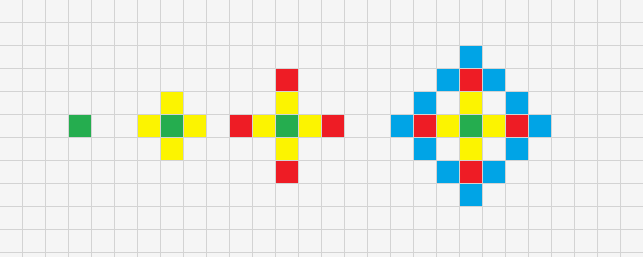
\includegraphics[width=0.72\textwidth]{squares lateral 4 gen.png}
\caption{Négyzetes rács (oldalszomszédság), 4. generációs állapot}
\end{figure}

\begin{figure}[htbp]
\centering
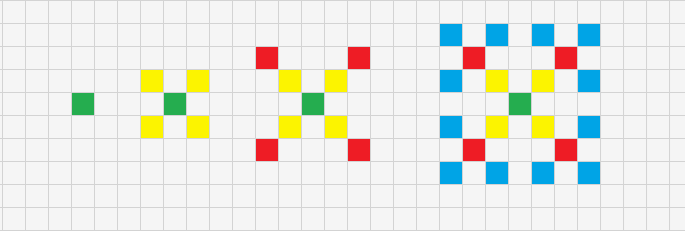
\includegraphics[width=0.72\textwidth]{squares apex 4 gen.png}
\caption{Négyzetes rács (átlós szomszédság), 4. generációs állapot}
\end{figure}

\begin{figure}[htbp]
\centering
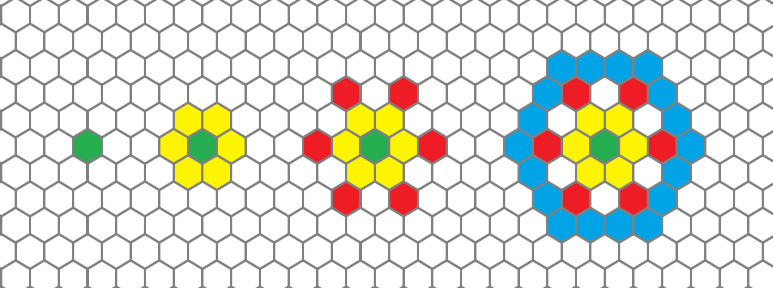
\includegraphics[width=0.72\textwidth]{hex 4 gen.png}
\caption{Hexagonális rács, 4. generációs állapot}
\end{figure}

\subsubsection{Conway-féle életjáték (Game of Life) szabályai a programban}
A \textbf{Game of Life} a leggyakrabban használt klasszikus kétdimenziós sejtautomata. Szabályjelölése: \textbf{B3/S23} --- \textit{birth} ha pontosan 3 élő szomszéd, \textit{survival} ha 2 vagy 3 élő szomszéd (Moore-szomszédság, azaz a középponton kívüli nyolc szomszéd figyelembevétele).

\paragraph{Élő sejt túlélése.}
Egy élő sejt tovább él, ha 2 vagy 3 élő szomszédja van. Ha kevesebb mint 2 van, \textbf{alulnépesedés} miatt elpusztul; ha több mint 3, \textbf{túlnépesedés} miatt hal meg.

\paragraph{Halott sejt születése.}
Egy üres cella pontosan 3 élő szomszéd esetén válik élővé (születés).

\begin{table}[htbp]
\centering
\caption{Conway életjáték: állapotátmenetek összefoglaló táblázata}
\begin{tabular}{@{}lll@{}}
\toprule
\textbf{Jelenlegi állapot} & \textbf{Élő szomszédok száma} & \textbf{Következő állapot} \\
\midrule
élő & 2 vagy 3 & élő \\
élő & kevesebb mint 2 & halott (alulnépesedés) \\
élő & több mint 3 & halott (túlnépesedés) \\
halott & pontosan 3 & élő (születés) \\
halott & más eset & halott \\
\bottomrule
\end{tabular}
\end{table}

\section{Matematikai és informatikai jelentőség}
A sejtautomaták kiemelkedő jelentőséggel bírnak mind matematikai, mind informatikai szempontból, mivel egyszerű szabályrendszerekkel képesek összetett viselkedések modellezésére. Jól szemléltetik azt az alapelvet, hogy lokális kölcsönhatásokból globális mintázatok és szervezett struktúrák alakulhatnak ki. Emiatt a komplex rendszerek vizsgálatának egyik fontos eszközévé váltak.

Matematikai nézőpontból a sejtautomaták kapcsolatban állnak a diszkrét matematikával, a kombinatorikával, a gráfelmélettel és a dinamikus rendszerek elméletével. Vizsgálatuk során elemezhető a stabilitás, a periodicitás, a káoszszerű viselkedés, valamint a kezdeti feltételek érzékenysége. Egyes szabályrendszerek esetében kimutatható, hogy rendkívül egyszerű definíció mellett is nehezen előre jelezhető fejlődés alakul ki.

Informatikai szempontból a sejtautomaták különösen fontosak, mert természetes módon modellezik a párhuzamos működést. Minden cella egyszerre, azonos szabály alapján frissülhet, ezért a modell jól illeszthető többmagos processzorokhoz, grafikus gyorsítókhoz és elosztott rendszerekhez. Emiatt gyakran használják nagy számításigényű szimulációkban.

A számításelméletben is jelentős szerepük van, mivel bizonyos sejtautomaták univerzális számításra képesek. Ez azt jelenti, hogy megfelelő szabályrendszer mellett ugyanazokat a feladatokat is megvalósíthatják, mint egy általános célú számítógép. Ennek legismertebb példája a Wolfram-féle 110-es szabály.

Gyakorlati alkalmazásuk rendkívül széles körű: használják közlekedési modellekben, járványterjedés vizsgálatában, ökológiai rendszerek elemzésében, képfeldolgozásban, titkosítási eljárásokban, valamint oktatási célokra is. Vizualizálhatóságuk és könnyen értelmezhető működésük miatt kiváló eszközt jelentenek algoritmikus gondolkodás és modellezési szemlélet fejlesztésére.

A sejtautomaták egyik legnagyobb értéke, hogy egyszerű szabályokból kiindulva kapcsolják össze az elméleti modelleket és a gyakorlati, számítógépes megvalósítást.

\chapter{Technológiai áttekintés}

\section{Projektarchitektúra áttekintése}
A Cellauto rendszer jelenlegi architektúrája három, egymástól technológiailag elkülönített, de közös adat- és jogosultsági modellen működő komponensre épül: \texttt{api}, \texttt{admin} és \texttt{www}. Az \texttt{api} réteg Laravel 12 alapú REST szolgáltatásként \cite{laravel,laravel-releases} a központi üzleti logikát, a hitelesítést, a jogosultságkezelést és a perzisztenciát valósítja meg. Az \texttt{admin} kliens React + TypeScript alapú \cite{react,typescript-docs} üzemeltetői felület, amely mára nemcsak a felhasználó-, szólista- és színlista-kezelést tartalmazza, hanem a vizsgaeredmények részletes elemzését és a naplózási (audit) funkciókat is. A \texttt{www} komponens a végfelhasználói alkalmazás, amely publikus homokozó módban és bejelentkezett, feladatorientált módban egyaránt működik.

A bővítések hatására az architektúra hangsúlyosabb rétegszétválasztást követ: a kliensalkalmazások elsődlegesen megjelenítési és folyamatvezérlési feladatot látnak el, míg a szabályérvényesítés (jogosultság, validáció, tulajdonosi kontroll, konzisztencia) szerveroldalon történik. Ez a felépítés csökkenti a duplikált üzleti logikát, javítja a karbantarthatóságot, és lehetővé teszi, hogy új modulok (például vizsga-visszajelzés, naplóelemzés, mentési folyamatok) a meglévő API-szerződésre építve, kontrolláltan bővíthetők legyenek.

\section{Backend technológia (\texttt{api})}
A backend komponens technológiai szempontból egy API-first szemléletű, REST alapú szolgáltatásréteg, amely a kliensalkalmazások (admin és \texttt{www}) számára biztosít hozzáférést az üzleti funkciókhoz és az adatokhoz. A kialakítás célja a stabil működés, a biztonságos hozzáférés és a fenntartható fejleszthetőség.

\paragraph{Alkalmazott technológiák.}
A megoldás PHP 8.2 futtatókörnyezetre \cite{php-docs} és Laravel 12 keretrendszerre \cite{laravel} épül. A Laravel biztosítja a routingot, a middleware-alapú kérésfeldolgozást, a validációt, az egységes hibakezelést és az ORM-integrációt. A védett végpontok hitelesítése Laravel Sanctum tokenekkel \cite{sanctum} történik, amelyet egyedi \texttt{active-session} middleware egészít ki a munkamenet- és státuszellenőrzéshez.

\paragraph{Adatkezelés és perzisztencia.}
Az adatelérés Eloquent ORM modelleken \cite{eloquent-orm} keresztül történik, amelyek a relációkat és a típuskonverziókat is definiálják. Az adatbázisséma verziózott migrációkkal kezelt, ezért a sémaváltozások reprodukálhatóan telepíthetők különböző környezetekben is. Ez különösen fontos olyan többmodulos rendszerben, ahol a felhasználói, listakezelési, mentési és értékelési entitások erősen összekapcsolódnak.

\paragraph{Kommunikációs és architekturális modell.}
Az API erőforrás-alapú végpontokra (\texttt{/api/...}) és szabványos HTTP metódusokra (\texttt{GET}, \texttt{POST}, \texttt{PUT}, \texttt{DELETE}) épül. A kliens-szerver kommunikáció JSON formátumban \cite{json-org} zajlik, tipikusan\\
\path{Accept: application/json} és \path{Content-Type: application/json} fejlécekkel.

Technológiai nézőpontból a backend rétegezett szerkezetet követ: route $\rightarrow$ middleware $\rightarrow$ controller $\rightarrow$ model $\rightarrow$ adatbázis. Ez a felépítés jól skálázható, könnyen karbantartható, és lehetővé teszi a jogosultsági szabályok, valamint az üzleti logika központi érvényesítését.

\paragraph{Robusztusság és fejlesztési támogatás.}
A backend a Laravel validációs és kivételkezelési mechanizmusaira támaszkodik, ezért a hibák strukturált JSON válaszokban jelennek meg (\texttt{error}, \texttt{message}, \texttt{errors}). Ez segíti a frontend differenciált hibaágkezelését.

A minőségbiztosítást és a fejlesztési folyamatot olyan eszközök támogatják, mint a PHPUnit (tesztelés), a Laravel Pint (kódformázás és stílusellenőrzés), valamint a Laravel Tinker (interaktív fejlesztői vizsgálat). Ennek eredményeként a backend fejlesztése kontrollált, automatizálható és hosszú távon fenntartható.

\paragraph{Fejlesztői környezet.}
A fejlesztés során elsődleges IDE-ként a Visual Studio Code (VS Code) került használatra. Az egységes szerkesztői környezet támogatta a backend és frontend komponensek párhuzamos fejlesztését, valamint a gyors hibakeresést és refaktorálást.

\section{Frontend technológiák}

\subsection{Admin felület}
Az admin felület modern, komponensalapú webalkalmazásként készült. A kliensoldali technológiai alapot a React 19 \cite{react,react-19-blog}, a TypeScript \cite{typescript-docs} és a Vite \cite{vite-guide} adja: a React a felület komponensstruktúráját és állapotkezelését támogatja, a TypeScript típusossága javítja a karbantarthatóságot, a Vite pedig gyors fejlesztői futtatást és build-folyamatot biztosít. A böngészős renderelést a React DOM végzi, a megjelenést pedig egyedi, kézzel írt CSS stílusok szabályozzák \cite{css3-roadmap}.

Az admin kliens a backenddel HTTP alapú JSON kommunikáción keresztül kapcsolódik (\texttt{fetch} hívásokkal). Fejlesztői környezetben a Vite proxy a \texttt{/api} útvonalat a Laravel API felé továbbítja, ami egyszerűsíti az integrációs működést.

Minőségbiztosítási oldalon az admin frontendnél az ESLint \cite{eslint-docs} és a TypeScript fordító (\texttt{tsc}) \cite{typescript-docs} biztosítja a statikus ellenőrzést, míg a backend oldali kapcsolódó fejlesztést PHPUnit és Laravel Pint támogatja.

\subsection{Felhasznlói felület (\texttt{www})}
A \texttt{www} frontend a klasszikus webes technológiákra épül: HTML5 \cite{html5-spec} adja az oldalstruktúrát, CSS3 \cite{css3-roadmap} a megjelenést, a kliensoldali üzleti logikát pedig moduláris, keretrendszerfüggetlen JavaScript valósítja meg. A felület kezeli többek között a táblaállapot-műveleteket, valamint a gyakorlási és vizsgafolyamatok kliensoldali vezérlését.

A helyi fejlesztésnél a PHP beépített szervere \cite{php-docs} (\texttt{php -S}) szolgál statikus kiszolgálásra, a \texttt{router.php} alapú proxylogika pedig az \texttt{/api/*} hívásokat továbbítja a Laravel backend felé (cURL \cite{curl-docs} használatával). Ennek célja, hogy fejlesztéskor a frontend és az API egységes host/port alatt legyen elérhető, így a CORS-kezelés egyszerűbbé válik.

A \texttt{www} kliens és a backend közötti kommunikáció HTTP/HTTPS és JSON \cite{json-org} alapon történik, a védett végpontoknál Bearer tokenes hitelesítéssel. Az architektúra rétegezett: prezentációs réteg (HTML/CSS/JavaScript), alkalmazáslogikai és API-réteg (Laravel \cite{laravel}), valamint adatperzisztencia-réteg (relációs adatbázis, fejlesztésben alapértelmezetten SQLite). Ez a felépítés jól támogatja a későbbi bővítéseket és a hosszú távú karbantarthatóságot.

\section{Adatbázis és perzisztencia}
A rendszer backend komponense relációs adatbázisra épülő perzisztenciát valósít meg. A perzisztencia célja, hogy az alkalmazás üzleti objektumai (felhasználók, listák, mentések, értékelések, naplóbejegyzések) konzisztens, visszakereshető és tranzakcióbiztos módon tárolódjanak.

\paragraph{Adatbázis-modell alapelvei.}
A projekt adatmodellje relációs szemléletet követ, ahol a központi entitás a \texttt{users} tábla, a domain-specifikus táblák idegen kulcsokon keresztül ehhez és egymáshoz kapcsolódnak, és az 1:N kapcsolatok dominálnak (például felhasználó $\rightarrow$ listák, csoport $\rightarrow$ mentések). Több helyen összerendelő jellegű relációk is megjelennek (például szókapcsolatok, feladatértékelések), ami támogatja az üzleti logika természetes adatbázis-szintű leképezését.

\paragraph{Sémakezelés és verziókövetés.}
Az adatbázis-séma Laravel migrációkkal kezelt \cite{laravel}. Ez biztosítja a struktúra verziózott nyomon követhetőségét, a fejlesztői és éles környezetek közötti reprodukálhatóságot, valamint a kontrollált, szükség esetén visszagörgethető sémamódosításokat.

\paragraph{Perzisztencia az alkalmazásrétegben.}
Az alkalmazás Eloquent ORM-et \cite{eloquent-orm} használ:
\begin{itemize}
  \item modellek reprezentálják a táblákat;
  \item relációk deklarálhatók (\texttt{belongsTo}, \texttt{hasMany});
  \item mezőszintű típuskonverziók adhatók meg (\texttt{casts}, például \texttt{array}, \texttt{datetime},\\ \texttt{integer});
  \item egységes API áll rendelkezésre az adatbázis-műveletekhez.
\end{itemize}

Ennek eredményeként a perzisztencia réteg jól olvashatóan és karbantartható módon integrálódik az üzleti logikába.

\paragraph{Adatintegritás és konzisztencia.}
Az adatintegritást több szint együttesen biztosítja:
\begin{enumerate}
  \item adatbázisszintű korlátok (elsődleges kulcsok, idegen kulcsok, egyedi indexek, \texttt{ON DELETE} szabályok);
  \item alkalmazásszintű validáció (kötelező mezők, típuskényszerek, üzleti szabályok);
  \item tranzakciókezelés a több lépéses műveletek atomi végrehajtásához.
\end{enumerate}

\paragraph{JSON mezők és auditálhatóság.}
A projekt bizonyos dinamikus szerkezetű tartalmakat JSON mezőkben \cite{json-org} tárol (például mentett táblaállapot vagy kitöltött feladatállapot). Ez a hibrid megközelítés megtartja a relációs modell előnyeit, miközben rugalmasan kezeli a változó belső adatszerkezeteket.

A hozzáférési események (látogatás, bejelentkezés, kijelentkezés) külön táblában tárolódnak, ami támogatja az utólagos elemzést és hibakeresést, növeli az átláthatóságot biztonsági és üzemeltetési szempontból, és auditfunkciót biztosít.

\section{API-szerződés és kommunikációs elvek}
Az alkalmazás kliens--szerver kommunikációja REST szemléletű HTTP API-n keresztül valósul meg, egységes \texttt{/api} útvonal-előtaggal. Az API-szerződés célja, hogy stabil, egyértelmű és bővíthető interfészt biztosítson a frontend és backend komponensek között.

\paragraph{Adatformátum és kommunikációs alapelvek.}
A kommunikáció JSON formátumban történik, alapértelmezett fejlécekkel (\texttt{Accept:}\\ \texttt{application/json}, \texttt{Content-Type: application/json}). Hitelesített hívások esetén a kliens Sanctum Bearer tokent használ.

Az API erőforrás-orientált végpontstruktúrát követ, ahol az URI-k a domain objektumokat reprezentálják, a HTTP metódusok (\texttt{GET}, \texttt{POST}, \texttt{PUT}, \texttt{DELETE}) pedig a műveleti szándékot fejezik ki. A beágyazott útvonalak az összetartozó adatok relációját jelzik (például lista $\rightarrow$ szavak, csoport $\rightarrow$ mentések).

\paragraph{Hitelesítési és jogosultsági szerződés.}
A végpontok három fő jogosultsági rétegre bonthatók:
\begin{enumerate}
  \item nyilvános végpontok (például \path{POST /api/login}, \path{GET /api/ping},\\ \path{POST /api/access-logs/visit});
  \item hitelesített felhasználói végpontok (\texttt{auth:sanctum} + \texttt{active-session});
  \item emelt jogosultságú végpontok (\texttt{staff}, illetve \texttt{admin} middleware).
\end{enumerate}

Az \texttt{active-session} middleware a token érvényességén túl a felhasználó állapotát (aktív/felfüggesztett) és az inaktivitási időkorlátot is ellenőrzi, így a hozzáférésvezérlés nem pusztán tokenlétezésre épül.

\paragraph{Válaszok és hibakezelés.}
A válaszok egységesen JSON formátumban érkeznek. Sikeres műveleteknél az API tipikusan \texttt{201 Created} (létrehozás), \texttt{200 OK} (lekérdezés/módosítás), illetve \texttt{200 OK} státuszobjektumot (törlés) használ.

A hibakezelés robusztusan kezeli az eltérő válaszstruktúrákat: \texttt{error}, \texttt{message}, \texttt{errors}. Ez heterogén hibaformátum mellett is stabil kliensműködést tesz lehetővé.

\paragraph{Kulcsfontosságú végpontcsoportok.}
Az aktuális szerződés fő funkcionális blokkjai: auth és session, felhasználók és adminisztráció, szólisták és szavak, generációs üzenetek és szókapcsolatok, színlisták és színek, táblaállapot-mentések, feladatmentések és értékelések, staff nézetek, valamint naplózási végpontok.

A kommunikációs konzisztenciát az egységes URI- és metóduskonvenciók, a middleware\allowbreak-alapú rétegzett hozzáférésvédelem, a relációt kifejező beágyazott útvonalak és a géppel jól feldolgozható JSON válaszstruktúra együtt biztosítják.

\section{Részletes API híváslista}
Az alkalmazás REST szemléletű HTTP API-t kínál; minden végpont az \texttt{/api} előtaggal érhető el (példa: \texttt{GET /api/ping}). Az alábbi összefoglaló az aktuális \texttt{api\_vegpontok} dokumentáció alapján készült.

\paragraph{Közös megjegyzések.}
A kommunikáció JSON formátumban történik (\texttt{Accept} és \texttt{Content-Type}: \texttt{application/json}). A védett hívások Sanctum Bearer tokennel azonosítanak. A middleware-lánc tipikusan \texttt{auth:sanctum} és \texttt{active-session}; emelt jogosultságnál \texttt{staff} illetve \texttt{admin}. Az \texttt{active-session} middleware az érvényes token mellett a felhasználó aktív státuszát és az inaktivitási időkorlátot is ellenőrzi.

\subsection{Nyilvános végpontok}
\small
\begin{longtable}{>{\raggedright\arraybackslash}p{0.40\textwidth}>{\raggedright\arraybackslash}p{0.12\textwidth}>{\raggedright\arraybackslash}p{0.42\textwidth}}
\toprule
\textbf{Végpont} & \textbf{Metódus} & \textbf{Leírás} \\
\midrule
\path{/api/ping} & GET & Egészség-/elérhetőség ellenőrzés (\texttt{ok}, \texttt{message}). \\[4pt]
\path{/api/login} & POST & Bejelentkezés: body \texttt{login}, \texttt{password}, \texttt{entry\_point} (\texttt{www} vagy \texttt{admin}); válasz: token és felhasználó. \\[4pt]
\path{/api/access-logs/visit} & POST & Látogatási esemény naplózása (nem feltétlenül bejelentkezett felhasználótól). \\[4pt]
\bottomrule
\end{longtable}
\normalsize

\subsection{Bejelentkezett felhasználó (\texttt{auth:sanctum} + \texttt{active-session})}

\subsubsection*{Munkamenet és felhasználó}
\small
\begin{longtable}{>{\raggedright\arraybackslash}p{0.40\textwidth}>{\raggedright\arraybackslash}p{0.12\textwidth}>{\raggedright\arraybackslash}p{0.42\textwidth}}
\toprule
\textbf{Végpont} & \textbf{Metódus} & \textbf{Leírás} \\
\midrule
\path{/api/logout} & POST & Kijelentkezés; body: \texttt{entry\_point} (\texttt{www} vagy \texttt{admin}); aktuális token törlése. \\[4pt]
\path{/api/user} & GET & Bejelentkezett felhasználó adatai. \\[4pt]
\path{/api/users} & GET & Felhasználók listája (alkalmazás logikája szerint). \\[4pt]
\path{/api/access-logs/me} & GET & Saját hozzáférési naplóbejegyzések. \\[4pt]
\bottomrule
\end{longtable}
\normalsize

\subsubsection*{Szólisták}
\small
\begin{longtable}{>{\raggedright\arraybackslash}p{0.40\textwidth}>{\raggedright\arraybackslash}p{0.12\textwidth}>{\raggedright\arraybackslash}p{0.42\textwidth}}
\toprule
\textbf{Végpont} & \textbf{Metódus} & \textbf{Leírás} \\
\midrule
\path{/api/lists} & GET & A bejelentkezett felhasználó saját listái. \\[4pt]
\path{/api/public-lists} & GET & Nyilvános listák más felhasználóktól. \\[4pt]
\path{/api/lists} & POST & Új lista (\texttt{name}, opcionálisan \texttt{public}, \texttt{notes}, \texttt{wordlist}). \\[4pt]
\path{/api/lists/{list}} & GET & Egy lista részletei (olvasás: saját vagy nyilvános lista). \\[4pt]
\path{/api/lists/{list}} & PUT & Lista módosítása (csak tulajdonos). \\[4pt]
\path{/api/lists/{list}} & DELETE & Lista törlése (csak tulajdonos). \\[4pt]
\bottomrule
\end{longtable}
\normalsize

\subsubsection*{Szavak és generációk}
\small
\begin{longtable}{>{\raggedright\arraybackslash}p{0.40\textwidth}>{\raggedright\arraybackslash}p{0.12\textwidth}>{\raggedright\arraybackslash}p{0.42\textwidth}}
\toprule
\textbf{Végpont} & \textbf{Metódus} & \textbf{Leírás} \\
\midrule
\path{/api/lists/{list}/words} & GET & Szavak generációk szerint csoportosítva (JSON struktúra). \\[4pt]
\path{/api/lists/{list}/words} & POST & Új szó hozzáadása egy generációhoz (csak tulajdonos). \\[4pt]
\path{/api/lists/{list}/words/{word}} & PUT & Szó módosítása (csak tulajdonos). \\[4pt]
\path{/api/lists/{list}/words/{word}} & DELETE & Szó törlése (csak tulajdonos). \\[4pt]
\path{/api/lists/{list}/word-generations} & PUT & Teljes generációs struktúra felülírása (csak tulajdonos). \\[4pt]
\bottomrule
\end{longtable}
\normalsize

\newpage
\subsubsection*{Generációs üzenetek}
\small
\begin{longtable}{>{\raggedright\arraybackslash}p{0.40\textwidth}>{\raggedright\arraybackslash}p{0.12\textwidth}>{\raggedright\arraybackslash}p{0.42\textwidth}}
\toprule
\textbf{Végpont} & \textbf{Metódus} & \textbf{Leírás} \\
\midrule
\path{/api/lists/{list}/word-gen-messages} & GET & Üzenetek listája generációnként. \\[4pt]
\path{/api/lists/{list}/word-gen-messages} & PUT & Üzenetek felülírása (csak tulajdonos). \\[4pt]
\bottomrule
\end{longtable}
\normalsize

\subsubsection*{Szókapcsolatok (GEN\textit{n} $\rightarrow$ GEN\textit{n}+1)}
\small
\begin{longtable}{>{\raggedright\arraybackslash}p{0.40\textwidth}>{\raggedright\arraybackslash}p{0.12\textwidth}>{\raggedright\arraybackslash}p{0.42\textwidth}}
\toprule
\textbf{Végpont} & \textbf{Metódus} & \textbf{Leírás} \\
\midrule
\path{/api/lists/{list}/word-relations} & GET & Kapcsolatok listája; opcionális query: \texttt{from\_generation}. \\[4pt]
\path{/api/lists/{list}/word-relations} & POST & Új kapcsolat (\texttt{from\_word\_id}, \texttt{to\_word\_id}). \\[4pt]
\path{/api/lists/{list}/word-relations/from/{fromWord}} & PUT & Egy kiinduló szó összes kimenő kapcsolatának cseréje (\texttt{to\_word\_ids}). \\[4pt]
\path{/api/lists/{list}/word-relations/{relation}} & DELETE & Kapcsolat törlése. \\[4pt]
\bottomrule
\end{longtable}
\normalsize

\subsubsection*{Színlisták és színek}
\small
\begin{longtable}{>{\raggedright\arraybackslash}p{0.40\textwidth}>{\raggedright\arraybackslash}p{0.12\textwidth}>{\raggedright\arraybackslash}p{0.42\textwidth}}
\toprule
\textbf{Végpont} & \textbf{Metódus} & \textbf{Leírás} \\
\midrule
\path{/api/color-lists} & GET & Saját színlisták. \\[4pt]
\path{/api/color-lists} & POST & Új színlista (\texttt{name}). \\[4pt]
\path{/api/color-lists/{color\_list}} & GET & Egy színlista + színek (csak tulajdonos). \\[4pt]
\path{/api/color-lists/{color\_list}} & PUT & Színlista módosítása. \\[4pt]
\path{/api/color-lists/{color\_list}} & DELETE & Színlista törlése (színek is). \\[4pt]
\path{/api/color-lists/{color\_list}/colors} & GET & Színek listája. \\[4pt]
\path{/api/color-lists/{color\_list}/colors} & POST & Új szín (\texttt{color}, \texttt{position}). \\[4pt]
\path{/api/color-lists/{color\_list}/colors/{color}} & PUT & Szín módosítása. \\[4pt]
\path{/api/color-lists/{color\_list}/colors/{color}} & DELETE & Szín törlése. \\[4pt]
\bottomrule
\end{longtable}
\normalsize

\subsubsection*{Táblaállapot mentések (Laravel \texttt{apiResource})}
\small
\begin{longtable}{>{\raggedright\arraybackslash}p{0.40\textwidth}>{\raggedright\arraybackslash}p{0.12\textwidth}>{\raggedright\arraybackslash}p{0.42\textwidth}}
\toprule
\textbf{Végpont} & \textbf{Metódus} & \textbf{Leírás} \\
\midrule
\path{/api/board-save-groups} & \shortstack[l]{GET\\POST} & Mentéscsoportok; új csoport. \\[4pt]
\path{/api/board-save-groups/{board\_save\_group}} & \shortstack[l]{GET\\PUT\\DELETE} & Egy csoport; módosítás; törlés. \\[4pt]
\path{/api/board-save-groups/{board\_save\_group}/saves} & \shortstack[l]{GET\\POST} & Csoport mentései; új mentés. \\[4pt]
\path{/api/board-save-groups/{board\_save\_group}/saves/{save}} & \shortstack[l]{GET\\PUT\\DELETE} & Egy mentés olvasása, módosítása, törlése. \\[4pt]
\bottomrule
\end{longtable}
\normalsize

\subsubsection*{Feladatmentések és értékelések}
A feladatmentés-csoportok és mentések szintén \texttt{apiResource} szerkezetben érhetők el.

\small
\begin{longtable}{>{\raggedright\arraybackslash}p{0.40\textwidth}>{\raggedright\arraybackslash}p{0.12\textwidth}>{\raggedright\arraybackslash}p{0.42\textwidth}}
\toprule
\textbf{Végpont} & \textbf{Metódus} & \textbf{Leírás} \\
\midrule
\path{/api/task-save-groups} & \shortstack[l]{GET\\POST} & Feladatmentés-csoportok; új csoport. \\[4pt]
\path{/api/task-save-groups/{task\_save\_group}} & \shortstack[l]{GET\\PUT\\DELETE} & Egy csoport; módosítás; törlés. \\[4pt]
\path{/api/task-save-groups/{task\_save\_group}/saves} & \shortstack[l]{GET\\POST} & Csoport feladatmentései; új feladatmentés. \\[4pt]
\path{/api/task-save-groups/{task\_save\_group}/saves/{save}} & \shortstack[l]{GET\\PUT\\DELETE} & Egy feladatmentés olvasása, módosítása, törlése. \\[4pt]
\bottomrule
\end{longtable}
\normalsize

\newpage
Értékelések (a feladatmentés azonosítója a path-ban):

\small
\begin{longtable}{>{\raggedright\arraybackslash}p{0.40\textwidth}>{\raggedright\arraybackslash}p{0.12\textwidth}>{\raggedright\arraybackslash}p{0.42\textwidth}}
\toprule
\textbf{Végpont} & \textbf{Metódus} & \textbf{Leírás} \\
\midrule
\path{/api/task-saves/{task\_save}/evaluations} & \shortstack[l]{GET\\POST} & Értékelések listája; új értékelés (láthatóság: tulajdonos/admin vs.\ saját). \\[4pt]
\path{/api/task-saves/{task\_save}/evaluations/{task\_evaluation}} & \shortstack[l]{PUT\\DELETE} & Értékelés módosítása vagy törlése. \\[4pt]
\bottomrule
\end{longtable}
\normalsize

\subsection{Staff jogosultság (\texttt{staff} middleware)}
\small
\begin{longtable}{>{\raggedright\arraybackslash}p{0.40\textwidth}>{\raggedright\arraybackslash}p{0.12\textwidth}>{\raggedright\arraybackslash}p{0.42\textwidth}}
\toprule
\textbf{Végpont} & \textbf{Metódus} & \textbf{Leírás} \\
\midrule
\path{/api/staff/task-evaluations} & GET & Értékelések listája oktatói/staff nézetben. \\[4pt]
\path{/api/staff/task-evaluations/{task\_evaluation}} & GET & Egy értékelés részletei. \\[4pt]
\bottomrule
\end{longtable}
\normalsize

\subsection{Admin jogosultság (\texttt{admin} middleware)}
\small
\begin{longtable}{>{\raggedright\arraybackslash}p{0.40\textwidth}>{\raggedright\arraybackslash}p{0.12\textwidth}>{\raggedright\arraybackslash}p{0.42\textwidth}}
\toprule
\textbf{Végpont} & \textbf{Metódus} & \textbf{Leírás} \\
\midrule
\path{/api/admin/users/online-status} & GET & Felhasználók online információi (token + utolsó napló). \\[4pt]
\path{/api/access-logs} & GET & Teljes hozzáférési napló. \\[4pt]
\path{/api/users} & POST & Új felhasználó létrehozása. \\[4pt]
\path{/api/users/{id}} & \shortstack[l]{PUT\\DELETE} & Felhasználó módosítása vagy törlése (korlátozásokkal). \\[4pt]
\path{/api/users/{id}/suspend} & POST & Felhasználó felfüggesztése. \\[4pt]
\path{/api/users/{id}/unsuspend} & POST & Felfüggesztés feloldása. \\[4pt]
\bottomrule
\end{longtable}
\normalsize


\newpage
\subsection{Válasz- és hibakezelési elvek}
A rendszerben tipikusan az alábbi státuszkódok jelennek meg:
\begin{itemize}
  \item \textbf{200/201}: sikeres lekérés vagy létrehozás;
  \item \textbf{401}: hitelesítési hiba (érvénytelen vagy hiányzó token);
  \item \textbf{403}: jogosultsági hiba (nem megfelelő szerepkör vagy tulajdon);
  \item \textbf{404}: nem létező erőforrás vagy hibás összerendelés;
  \item \textbf{422}: validációs hiba (pl. duplikált név vagy pozíció).
\end{itemize}

\chapter{Rendszerterv a Cellauto projekthez}

\section{A rendszer célja és hatóköre}
A Cellauto célja egy olyan webes oktatási platform létrehozása volt, amely a sejtautomaták működését nemcsak bemutatja, hanem tanulási helyzetben is használhatóvá teszi. A rendszer tervezésekor fontos szempont volt, hogy ne csak demonstrációs felület legyen, hanem bővíthető, valódi oktatási helyzetekben is alkalmazható digitális környezet. A gyakorlatban ez a vizuális modellezés, a feladatalapú gyakorlás és a tanári-adminisztratív kezelés együttes megvalósítását jelenti.

A rendszer hatóköre több, egymástól funkcionálisan elkülönülő, mégis szorosan együttműködő komponensre terjed ki. A végfelhasználói felület biztosítja a sejtautomata\allowbreak-szimulációk futtatását, a feladatok végrehajtását és az eredmények megjelenítését, míg az adminisztrációs felület a háttérben szükséges tartalom- és felhasználókezelési műveletekért felel. A backend szolgáltatási réteg egységes API-n keresztül kapcsolja össze a két kliensoldali környezetet, és garantálja az üzleti logika, az adatkonzisztencia és a jogosultsági szabályok központi érvényesítését.

A célrendszer fő felhasználói csoportjai a diákok, a tanárok és az adminisztrátorok. A diákok számára a rendszer interaktív, visszajelzésalapú tanulási élményt nyújt, amely segíti a logikus gondolkodás, a problémamegoldó képesség és a kreativitás fejlődését. A tanárok és adminisztrátorok számára a platform olyan menedzsmentfunkciókat biztosít, amelyekkel kezelhetők a felhasználók, a szólisták, a színlisták, valamint a tanulási folyamatot támogató erőforrások. A szerepkörök világos szétválasztása a rendszertervezés egyik alapelve, amelyet kliensoldali és szerveroldali jogosultságkezelés együttesen érvényesít.

A funkcionális hatókörbe tartozik a hitelesítés és hozzáférés-ellenőrzés, az oktatási tartalmak kezelése, a szimulációs állapotok mentése és visszatöltése, továbbá az eredmények nyomon követése és értelmezhető visszajelzése. A rendszer emellett támogatja az egységes adatkezelést és a reprodukálható működést, ami különösen fontos oktatási és értékelési környezetben. A tervezés során hangsúlyos szempont volt, hogy a Cellauto később további modulokkal is bővíthető legyen anélkül, hogy az alaparchitektúra újratervezése szükségessé válna.

A hatókör tudatos lehatárolása érdekében rögzíthető, hogy a jelen fejlesztési fázis nem terjed ki natív mobilalkalmazás készítésére, teljes offline működés támogatására vagy valós idejű, többfelhasználós közös szerkesztésre. Ezek a lehetőségek jövőbeli továbbfejlesztési irányként jelennek meg, de nem részei a dolgozatban bemutatott kötelező rendszerfunkcióknak. A jelenlegi cél egy stabilan működő, jól dokumentált, oktatási célokra közvetlenül használható és technológiailag fenntartható webes rendszer bemutatása.

\section{Szerepkör- és jogosultsági modell}
A Cellauto rendszer jogosultsági modelljének célja, hogy a különböző felhasználói csoportok számára kizárólag a szerepkörüknek megfelelő funkciók legyenek elérhetők. A modell kialakításának alapelve a minimálisan szükséges jogosultság elve, vagyis minden felhasználó csak azokhoz az adatokhoz és műveletekhez férhet hozzá, amelyek a feladatai ellátásához feltétlenül szükségesek.

A rendszer négy alapvető szerepkört különböztet meg: \texttt{vendeg}, \texttt{diak}, \texttt{tanar} és \texttt{admin}. A \texttt{vendeg} szerepkör korlátozott hozzáférést biztosít, elsősorban nyilvános vagy bemutató jellegű funkciókhoz. A \texttt{diak} szerepkör célja a tanulási folyamat támogatása: a felhasználó hozzáfér a számára kijelölt feladatokhoz, saját mentéseihez és személyes adataihoz, ugyanakkor nem végezhet rendszerszintű módosításokat. A \texttt{tanar} szerepkör a pedagógiai támogatáshoz szükséges kiterjesztett jogosultságokat adja, például oktatási tartalmak kezelését vagy tanulói teljesítmények nyomon követését. Az \texttt{admin} szerepkör rendelkezik teljes körű menedzsmentjoggal, beleértve a felhasználókezelést, a rendszerparaméterek adminisztrációját és a kritikus konfigurációs műveleteket.

A jogosultságkezelés két szinten valósul meg. Kliensoldalon a felület szerepkörfüggően jeleníti meg a menüpontokat és műveleti lehetőségeket, ezáltal javítja a használhatóságot és csökkenti a hibás műveletek esélyét. Szerveroldalon azonban minden védett végpont esetében kötelező jogosultságellenőrzés történik middleware és policy szabályok segítségével, így a kliensoldali korlátozások megkerülése esetén sem hajtható végre jogosulatlan művelet.

A modell fontos eleme a tulajdonosi hozzáférés-ellenőrzés is. A felhasználóhoz kötött erőforrások (például mentések, egyéni listák, személyes adatok) esetében a rendszer nemcsak a szerepkört vizsgálja, hanem azt is, hogy az adott rekord a műveletet kezdeményező felhasználóhoz tartozik-e. Ez az elv megakadályozza az idegen adatokhoz való jogosulatlan hozzáférést, és biztosítja az adatvédelem követelményeinek érvényesülését.

A Cellauto szerepkör- és jogosultsági modellje a gyakorlatban bevált: egyszerre maradt kezelhető a felhasználóknak, és biztonságos az üzemeltetési oldalról.

\section{Részletes funkcionális követelmények}
A Cellauto rendszer funkcionális követelményei azt határozzák meg, hogy a platform milyen szolgáltatásokat nyújt a különböző felhasználói szerepkörök számára, és ezek milyen szabályok mentén működnek. A követelmények kialakításának alapelve, hogy minden művelet egyértelműen kapcsolódjon szerepkörhöz, jogosultsághoz és ellenőrizhető rendszerreakcióhoz. A rendszer így nem pusztán adatkezelést végez, hanem teljes oktatási folyamatokat támogat a feladat-összeállítástól a megoldáson át az értékelésig.

\subsection{Autentikáció és munkamenet-kezelés}

A rendszer biztosítja a felhasználók hitelesítését felhasználónév vagy e-mail cím és jelszó alapú bejelentkezéssel. Sikeres autentikáció után a kliens tokenalapú munkamenetet kezel, és szerepkörfüggő felületet jelenít meg. Követelmény, hogy oldalfrissítés esetén is visszaállítható legyen a bejelentkezett állapot, kijelentkezéskor pedig minden védett művelethez tartozó hozzáférés megszűnjön.

\subsection{Felhasználókezelés}

Az adminisztrációs felület támogatja a felhasználók listázását, keresését, létrehozását, szerkesztését, törlését, felfüggesztését és visszaaktiválását. A rendszernek biztosítania kell, hogy a jogosultsági állapotok változása azonnal érvényesüljön, és a kliensoldali megjelenítés konzisztens maradjon a szerveroldali adatokkal.

\subsection{Szólisták és színlisták kezelése}

A rendszer támogatja a szólisták és színlisták létrehozását, módosítását, törlését és rendezését. Követelmény a duplikátumok kezelése, az elemek stabil sorrendjének biztosítása, valamint a szerkesztési műveletek konzisztens tárolása. A színlisták esetében a felvitel kontrollált, előre definiált készletből történik, amely csökkenti a hibás adatbevitel lehetőségét.

\subsection{Táblaállapot mentések és visszatöltés}

A platform lehetőséget ad sejtautomata-állapotok mentésére és visszaállítására strukturált, JSON-alapú formában. A mentések felhasználói kontextusban kezeltek, tulajdonosi ellenőrzéssel védettek, így minden felhasználó csak a saját erőforrásait érheti el. A mentési funkció célja a reprodukálhatóság és a tanulási folyamat folytonosságának biztosítása.

\subsection{Gyakorló- és vizsgafeladatok összeállítása tanári oldalon}

A rendszer kiemelt funkciója, hogy a tanár önállóan állíthat össze feladatsorokat a diákok számára. A feladatok lehetnek:
\begin{itemize}
  \item kizárólag sejtautomata-alapú feladatok;
  \item kizárólag mondatképző (nyelvi) feladatok;
  \item a két feladattípus kombinációi egy közös feladatsorban.
\end{itemize}

A tanár a feladatokhoz nehézségi szintet rendelhet, így a tartalom differenciáltan igazítható a diákok tudásszintjéhez. Emellett vizsgamód esetén időkorlát is beállítható, amely meghatározza a rendelkezésre álló megoldási időt. Ez lehetővé teszi, hogy a rendszer ne csak gyakorlásra, hanem ellenőrzött számonkérésre is alkalmas legyen.

\subsection{Diákoldali feladathasználat és végrehajtás}

A diák a számára kiosztott feladatokat elérheti, megoldhatja és eredményeit visszajelzés formájában megtekintheti. Gyakorló módban a rendszer támogató működést és tanulást segítő visszacsatolást biztosít, vizsgamódban pedig a beállított időkorlát és szabályrendszer szerint, kontrollált környezetben történik a feladatmegoldás. Követelmény, hogy a hozzáférés, a feladatindítás, a beadás és az eredménykezelés szerepköralapon, megbízhatóan működjön.

\subsection{Funkcionális követelmények összegzése}

A funkcionális követelményrendszer akkor tekinthető teljesültnek, ha a tanári feladatösszeállítás, a diákoldali végrehajtás, a jogosultságkezelés és az adatkezelés egységesen, konzisztensen és reprodukálható módon működik. A kialakított struktúra célja, hogy a Cellauto stabil alapot adjon mind a napi gyakorláshoz, mind a vizsgáztatási folyamatok támogatásához.

\section{Nem-funkcionális követelmények}
A Cellauto rendszer nem-funkcionális követelményei a működés minőségi jellemzőit rögzítik. Ezek a követelmények nem közvetlenül új funkciókat írnak le, hanem azt határozzák meg, hogy a rendszer milyen biztonsági, teljesítménybeli, használhatósági és fenntarthatósági elvárások mellett tekinthető megfelelőnek.

\subsection{Biztonság}

A rendszer alapvető követelménye a biztonságos hozzáférés-vezérlés. A hitelesítés tokenalapon történik, és minden védett művelethez szerveroldali jogosultságellenőrzés tartozik. A szerepköralapú hozzáférés-szabályozás mellett a tulajdonosi ellenőrzés is kötelező, így a felhasználó kizárólag a saját erőforrásait érheti el és módosíthatja. Kiemelt elvárás továbbá, hogy jogosulatlan hozzáférési kísérlet esetén a rendszer egyértelmű, naplózható és biztonságos válasszal reagáljon.

\subsection{Adatkonzisztencia és megbízhatóság}

A rendszernek biztosítania kell az adatok konzisztens és ütközésmentes kezelését. Ennek feltétele a relációs integritási szabályok (idegen kulcsok, egyedi megszorítások) következetes alkalmazása, valamint az, hogy párhuzamos vagy ismételt műveletek esetén se jöhessen létre ellentmondásos állapot. A mentési és visszatöltési folyamatoknál külön követelmény a reprodukálhatóság, vagyis ugyanaz a mentett állapot azonos környezetben azonos eredménnyel visszaállítható legyen.

\subsection{Teljesítmény és skálázhatóság}

A rendszernek oktatási környezetben is stabil válaszidőt kell biztosítania, különösen a gyakran használt műveletek esetén (bejelentkezés, listázás, mentés, feladatindítás, beadás). Vizsgamódban kiemelt fontosságú, hogy időkorlátos feladatoknál a késleltetés ne torzítsa a felhasználói élményt és az értékelés megbízhatóságát. A kliens--szerver architektúra célja, hogy növekvő felhasználószám mellett is bővíthető és terhelhető maradjon a rendszer.

\subsection{Használhatóság és felhasználói élmény}

A felületnek egyértelmű, konzisztens és tanulást támogató működést kell nyújtania. Elvárás a magyar nyelvű, könnyen értelmezhető felhasználói kommunikáció, a műveletekhez tartozó azonnali visszajelzés, valamint a hibahelyzetek érthető kezelése. A gyakorló és vizsga folyamatokban különösen fontos, hogy a felhasználó mindig egyértelműen lássa az aktuális állapotot (pl. hátralévő idő, feladat típusa, beadási státusz).

\subsection{Karbantarthatóság és bővíthetőség}

A rendszer hosszú távú fenntarthatóságának feltétele a jól strukturált kódbázis, az elkülönített rétegek (frontend, backend, adatbázis) és a dokumentált API-szerződés. A sémafejlődés migrációalapon történik, ami biztosítja a változások kontrollálhatóságát és visszakövethetőségét. Követelmény, hogy új feladattípusok, értékelési szempontok vagy jogosultsági szabályok bevezetése minimális mellékhatással legyen megvalósítható.

\subsection{Összegzés}

A nem-funkcionális követelmények célja az volt, hogy a rendszer ne csak működjön, hanem biztonságos, stabil és hosszabb távon is fejleszthető maradjon. Ez egy oktatási platformnál különösen lényeges, mert ugyanazt a rendszert használják gyakorlásra és vizsgáztatásra is.

\section{Adatbázis-felépítés és magyarázat}
Az adatbázis kialakítása MySQL/InnoDB alapon \cite{mysql-docs} történt, célja a felhasználóközpontú adatelválasztás, a referenciális integritás és a rugalmas állapottárolás egyidejű biztosítása. A modell főként \texttt{users}-központú: a tartalmi és mentési entitások döntő többsége felhasználóhoz kötött.

\subsection{Főbb táblacsoportok}
\begin{itemize}
  \item \textbf{Szómodul:} \texttt{lists\_word}, \texttt{words}, \texttt{word\_gen\_messages}, \texttt{word\_relations}
  \item \textbf{Színmodul:} \texttt{color\_lists}, \texttt{colors}
  \item \textbf{Mentési modul:} \texttt{board\_save\_groups}, \texttt{board\_saves}, \texttt{task\_save\_groups}, \texttt{task\_saves}
  \item \textbf{Naplózás:} \texttt{access\_logs}
\end{itemize}

\subsection{Kapcsolatok és megszorítások}
A séma erős relációs integritással működik: az idegen kulcsok több helyen \texttt{ON DELETE CASCADE} viselkedéssel biztosítják, hogy törléskor ne maradjanak árva rekordok. Az egyedi kulcsok (például lista/sorrend vagy csoport/név kombinációk) konzisztens felhasználói rendezést és ütközésmentes mentéselnevezést garantálnak.

\subsection{MySQL deklarációk}
Az adatmodell fő tábláinak MySQL deklarációi a következők:

\begin{lstlisting}[style=mysqlstyle]
CREATE TABLE `users` (
  `id` BIGINT UNSIGNED NOT NULL AUTO_INCREMENT,
  `username` VARCHAR(255) NOT NULL,
  `name` VARCHAR(255) NOT NULL,
  `email` VARCHAR(255) NOT NULL,
  `role` VARCHAR(255) NOT NULL DEFAULT 'vendeg',
  `active` TINYINT(1) NOT NULL DEFAULT 1,
  `suspended_at` TIMESTAMP NULL DEFAULT NULL,
  `email_verified_at` TIMESTAMP NULL DEFAULT NULL,
  `password` VARCHAR(255) NOT NULL,
  `remember_token` VARCHAR(100) NULL DEFAULT NULL,
  `created_at` TIMESTAMP NULL DEFAULT NULL,
  `updated_at` TIMESTAMP NULL DEFAULT NULL,
  PRIMARY KEY (`id`),
  UNIQUE KEY `users_username_unique` (`username`),
  UNIQUE KEY `users_email_unique` (`email`)
) ENGINE=InnoDB DEFAULT CHARSET=utf8mb4 COLLATE=utf8mb4_unicode_ci;
\end{lstlisting}

\begin{lstlisting}[style=mysqlstyle]
CREATE TABLE `lists_word` (
  `id` BIGINT UNSIGNED NOT NULL AUTO_INCREMENT,
  `user_id` BIGINT UNSIGNED NOT NULL,
  `name` VARCHAR(255) NOT NULL,
  `public` TINYINT(1) NOT NULL DEFAULT 0,
  `notes` TEXT NULL,
  `wordlist` MEDIUMTEXT NULL,
  `created_at` TIMESTAMP NULL DEFAULT NULL,
  `updated_at` TIMESTAMP NULL DEFAULT NULL,
  PRIMARY KEY (`id`),
  KEY `lists_word_user_id_foreign` (`user_id`),
  CONSTRAINT `lists_word_user_id_foreign`
    FOREIGN KEY (`user_id`) REFERENCES `users` (`id`) ON DELETE CASCADE
) ENGINE=InnoDB DEFAULT CHARSET=utf8mb4 COLLATE=utf8mb4_unicode_ci;
\end{lstlisting}

\begin{lstlisting}[style=mysqlstyle]
CREATE TABLE `words` (
  `id` BIGINT UNSIGNED NOT NULL AUTO_INCREMENT,
  `list_id` BIGINT UNSIGNED NOT NULL,
  `generation` INT UNSIGNED NOT NULL DEFAULT 1,
  `word` VARCHAR(255) NOT NULL,
  `created_at` TIMESTAMP NULL DEFAULT NULL,
  `updated_at` TIMESTAMP NULL DEFAULT NULL,
  PRIMARY KEY (`id`),
  UNIQUE KEY `words_list_generation_word_unique` (`list_id`, `generation`, `word`),
  KEY `fk_words_list` (`list_id`),
  CONSTRAINT `fk_words_list`
    FOREIGN KEY (`list_id`) REFERENCES `lists_word` (`id`) ON DELETE CASCADE
) ENGINE=InnoDB DEFAULT CHARSET=utf8mb4 COLLATE=utf8mb4_unicode_ci;
\end{lstlisting}

\begin{lstlisting}[style=mysqlstyle]
CREATE TABLE `word_gen_messages` (
  `id` BIGINT UNSIGNED NOT NULL AUTO_INCREMENT,
  `list_id` BIGINT UNSIGNED NOT NULL,
  `generation` INT UNSIGNED NOT NULL,
  `correct_answer_message` TEXT NULL,
  `incorrect_answer_message` TEXT NULL,
  `created_at` TIMESTAMP NULL DEFAULT NULL,
  `updated_at` TIMESTAMP NULL DEFAULT NULL,
  PRIMARY KEY (`id`),
  UNIQUE KEY `word_gen_messages_list_generation_unique` (`list_id`, `generation`),
  KEY `word_gen_messages_list_id_foreign` (`list_id`),
  CONSTRAINT `word_gen_messages_list_id_foreign`
    FOREIGN KEY (`list_id`) REFERENCES `lists_word` (`id`) ON DELETE CASCADE
) ENGINE=InnoDB DEFAULT CHARSET=utf8mb4 COLLATE=utf8mb4_unicode_ci;
\end{lstlisting}

\begin{lstlisting}[style=mysqlstyle]
CREATE TABLE `word_relations` (
  `id` BIGINT UNSIGNED NOT NULL AUTO_INCREMENT,
  `list_id` BIGINT UNSIGNED NOT NULL,
  `from_word_id` BIGINT UNSIGNED NOT NULL,
  `to_word_id` BIGINT UNSIGNED NOT NULL,
  `created_at` TIMESTAMP NULL DEFAULT NULL,
  `updated_at` TIMESTAMP NULL DEFAULT NULL,
  PRIMARY KEY (`id`),
  UNIQUE KEY `word_relations_unique` (`list_id`, `from_word_id`, `to_word_id`),
  KEY `word_relations_list_id_from_word_id_index` (`list_id`, `from_word_id`),
  KEY `word_relations_list_id_to_word_id_index` (`list_id`, `to_word_id`),
  CONSTRAINT `word_relations_list_id_foreign`
    FOREIGN KEY (`list_id`) REFERENCES `lists_word` (`id`) ON DELETE CASCADE,
  CONSTRAINT `word_relations_from_word_id_foreign`
    FOREIGN KEY (`from_word_id`) REFERENCES `words` (`id`) ON DELETE CASCADE,
  CONSTRAINT `word_relations_to_word_id_foreign`
    FOREIGN KEY (`to_word_id`) REFERENCES `words` (`id`) ON DELETE CASCADE
) ENGINE=InnoDB DEFAULT CHARSET=utf8mb4 COLLATE=utf8mb4_unicode_ci;
\end{lstlisting}

\begin{lstlisting}[style=mysqlstyle]
CREATE TABLE `access_logs` (
  `id` BIGINT UNSIGNED NOT NULL AUTO_INCREMENT,
  `user_id` BIGINT UNSIGNED NULL,
  `event_type` VARCHAR(20) NOT NULL,
  `entry_point` VARCHAR(20) NOT NULL,
  `ip_address` VARCHAR(45) NOT NULL,
  `user_agent` VARCHAR(1024) NULL,
  `occurred_at` TIMESTAMP NOT NULL,
  `created_at` TIMESTAMP NULL DEFAULT NULL,
  `updated_at` TIMESTAMP NULL DEFAULT NULL,
  PRIMARY KEY (`id`),
  KEY `access_logs_event_type_entry_point_index` (`event_type`, `entry_point`),
  KEY `access_logs_occurred_at_index` (`occurred_at`),
  KEY `access_logs_user_id_index` (`user_id`),
  CONSTRAINT `access_logs_user_id_foreign`
    FOREIGN KEY (`user_id`) REFERENCES `users` (`id`) ON DELETE SET NULL
) ENGINE=InnoDB DEFAULT CHARSET=utf8mb4 COLLATE=utf8mb4_unicode_ci;
\end{lstlisting}

\begin{lstlisting}[style=mysqlstyle]
CREATE TABLE `color_lists` (
  `id` BIGINT UNSIGNED NOT NULL AUTO_INCREMENT,
  `user_id` BIGINT UNSIGNED NOT NULL,
  `name` VARCHAR(255) NOT NULL,
  `created_at` TIMESTAMP NULL DEFAULT NULL,
  `updated_at` TIMESTAMP NULL DEFAULT NULL,
  PRIMARY KEY (`id`),
  KEY `color_lists_user_id_foreign` (`user_id`),
  CONSTRAINT `color_lists_user_id_foreign`
    FOREIGN KEY (`user_id`) REFERENCES `users` (`id`) ON DELETE CASCADE
) ENGINE=InnoDB DEFAULT CHARSET=utf8mb4 COLLATE=utf8mb4_unicode_ci;
\end{lstlisting}

\begin{lstlisting}[style=mysqlstyle]
CREATE TABLE `colors` (
  `id` BIGINT UNSIGNED NOT NULL AUTO_INCREMENT,
  `list_id` BIGINT UNSIGNED NOT NULL,
  `color` VARCHAR(50) NOT NULL,
  `position` INT UNSIGNED NOT NULL,
  `created_at` TIMESTAMP NULL DEFAULT NULL,
  `updated_at` TIMESTAMP NULL DEFAULT NULL,
  PRIMARY KEY (`id`),
  UNIQUE KEY `colors_list_position_unique` (`list_id`, `position`),
  KEY `colors_list_id_foreign` (`list_id`),
  CONSTRAINT `colors_list_id_foreign`
    FOREIGN KEY (`list_id`) REFERENCES `color_lists` (`id`) ON DELETE CASCADE
) ENGINE=InnoDB DEFAULT CHARSET=utf8mb4 COLLATE=utf8mb4_unicode_ci;
\end{lstlisting}

\begin{lstlisting}[style=mysqlstyle]
CREATE TABLE `board_save_groups` (
  `id` BIGINT UNSIGNED NOT NULL AUTO_INCREMENT,
  `user_id` BIGINT UNSIGNED NOT NULL,
  `name` VARCHAR(255) NOT NULL,
  `position` INT UNSIGNED NULL,
  `created_at` TIMESTAMP NULL DEFAULT NULL,
  `updated_at` TIMESTAMP NULL DEFAULT NULL,
  PRIMARY KEY (`id`),
  KEY `board_save_groups_user_id_foreign` (`user_id`),
  CONSTRAINT `board_save_groups_user_id_foreign`
    FOREIGN KEY (`user_id`) REFERENCES `users` (`id`) ON DELETE CASCADE
) ENGINE=InnoDB DEFAULT CHARSET=utf8mb4 COLLATE=utf8mb4_unicode_ci;
\end{lstlisting}

\begin{lstlisting}[style=mysqlstyle]
CREATE TABLE `board_saves` (
  `id` BIGINT UNSIGNED NOT NULL AUTO_INCREMENT,
  `user_id` BIGINT UNSIGNED NOT NULL,
  `board_save_group_id` BIGINT UNSIGNED NOT NULL,
  `name` VARCHAR(255) NOT NULL,
  `payload` JSON NOT NULL,
  `created_at` TIMESTAMP NULL DEFAULT NULL,
  `updated_at` TIMESTAMP NULL DEFAULT NULL,
  PRIMARY KEY (`id`),
  UNIQUE KEY `board_saves_board_save_group_id_name_unique` (`board_save_group_id`, `name`),
  KEY `board_saves_user_id_foreign` (`user_id`),
  CONSTRAINT `board_saves_user_id_foreign`
    FOREIGN KEY (`user_id`) REFERENCES `users` (`id`) ON DELETE CASCADE,
  CONSTRAINT `board_saves_board_save_group_id_foreign`
    FOREIGN KEY (`board_save_group_id`) REFERENCES `board_save_groups` (`id`) ON DELETE CASCADE
) ENGINE=InnoDB DEFAULT CHARSET=utf8mb4 COLLATE=utf8mb4_unicode_ci;
\end{lstlisting}

\begin{lstlisting}[style=mysqlstyle]
CREATE TABLE `task_save_groups` (
  `id` BIGINT UNSIGNED NOT NULL AUTO_INCREMENT,
  `user_id` BIGINT UNSIGNED NOT NULL,
  `name` VARCHAR(255) NOT NULL,
  `position` INT UNSIGNED NULL,
  `created_at` TIMESTAMP NULL DEFAULT NULL,
  `updated_at` TIMESTAMP NULL DEFAULT NULL,
  PRIMARY KEY (`id`),
  KEY `task_save_groups_user_id_foreign` (`user_id`),
  CONSTRAINT `task_save_groups_user_id_foreign`
    FOREIGN KEY (`user_id`) REFERENCES `users` (`id`) ON DELETE CASCADE
) ENGINE=InnoDB DEFAULT CHARSET=utf8mb4 COLLATE=utf8mb4_unicode_ci;
\end{lstlisting}

\begin{lstlisting}[style=mysqlstyle]
CREATE TABLE `task_saves` (
  `id` BIGINT UNSIGNED NOT NULL AUTO_INCREMENT,
  `user_id` BIGINT UNSIGNED NOT NULL,
  `task_save_group_id` BIGINT UNSIGNED NOT NULL,
  `word_list_id` BIGINT UNSIGNED NULL,
  `name` VARCHAR(255) NOT NULL,
  `level` ENUM('Easy','Medium','Hard') NOT NULL DEFAULT 'Medium',
  `generation_mode` VARCHAR(50) NOT NULL,
  `board_size` INT UNSIGNED NOT NULL,
  `generations_count` INT UNSIGNED NOT NULL,
  `time_limit` INT UNSIGNED NOT NULL,
  `payload` JSON NOT NULL,
  `created_at` TIMESTAMP NULL DEFAULT NULL,
  `updated_at` TIMESTAMP NULL DEFAULT NULL,
  PRIMARY KEY (`id`),
  UNIQUE KEY `task_saves_group_name_unique` (`task_save_group_id`, `name`),
  KEY `task_saves_user_id_foreign` (`user_id`),
  KEY `task_saves_word_list_id_foreign` (`word_list_id`),
  CONSTRAINT `task_saves_user_id_foreign`
    FOREIGN KEY (`user_id`) REFERENCES `users` (`id`) ON DELETE CASCADE,
  CONSTRAINT `task_saves_task_save_group_id_foreign`
    FOREIGN KEY (`task_save_group_id`) REFERENCES `task_save_groups` (`id`) ON DELETE CASCADE,
  CONSTRAINT `task_saves_word_list_id_foreign`
    FOREIGN KEY (`word_list_id`) REFERENCES `lists_word` (`id`) ON DELETE SET NULL
) ENGINE=InnoDB DEFAULT CHARSET=utf8mb4 COLLATE=utf8mb4_unicode_ci;
\end{lstlisting}

\section{UML diagramok}\label{sec:uml-diagramok}
A rendszer adatmodelljének szemléltetésére két UML ábra készült. Az ábrák együtt mutatják a teljes relációs sémát, nem egyetlen, túlzsúfolt diagramon. A diagramokban szereplő fő táblák: \texttt{users}, \texttt{lists\_word}, \texttt{words}, \texttt{word\_gen\_messages}, \texttt{word\_relations}, \texttt{access\_logs}, \texttt{color\_lists}, \texttt{colors}, \texttt{board\_save\_groups}, \texttt{board\_saves}, \texttt{task\_save\_groups}, \texttt{task\_saves}. Az ábrák a táblák közötti kapcsolatokat, valamint a kulcs- és egyediségi viszonyokat szemléltetik.

\begin{figure}[htbp]
\centering
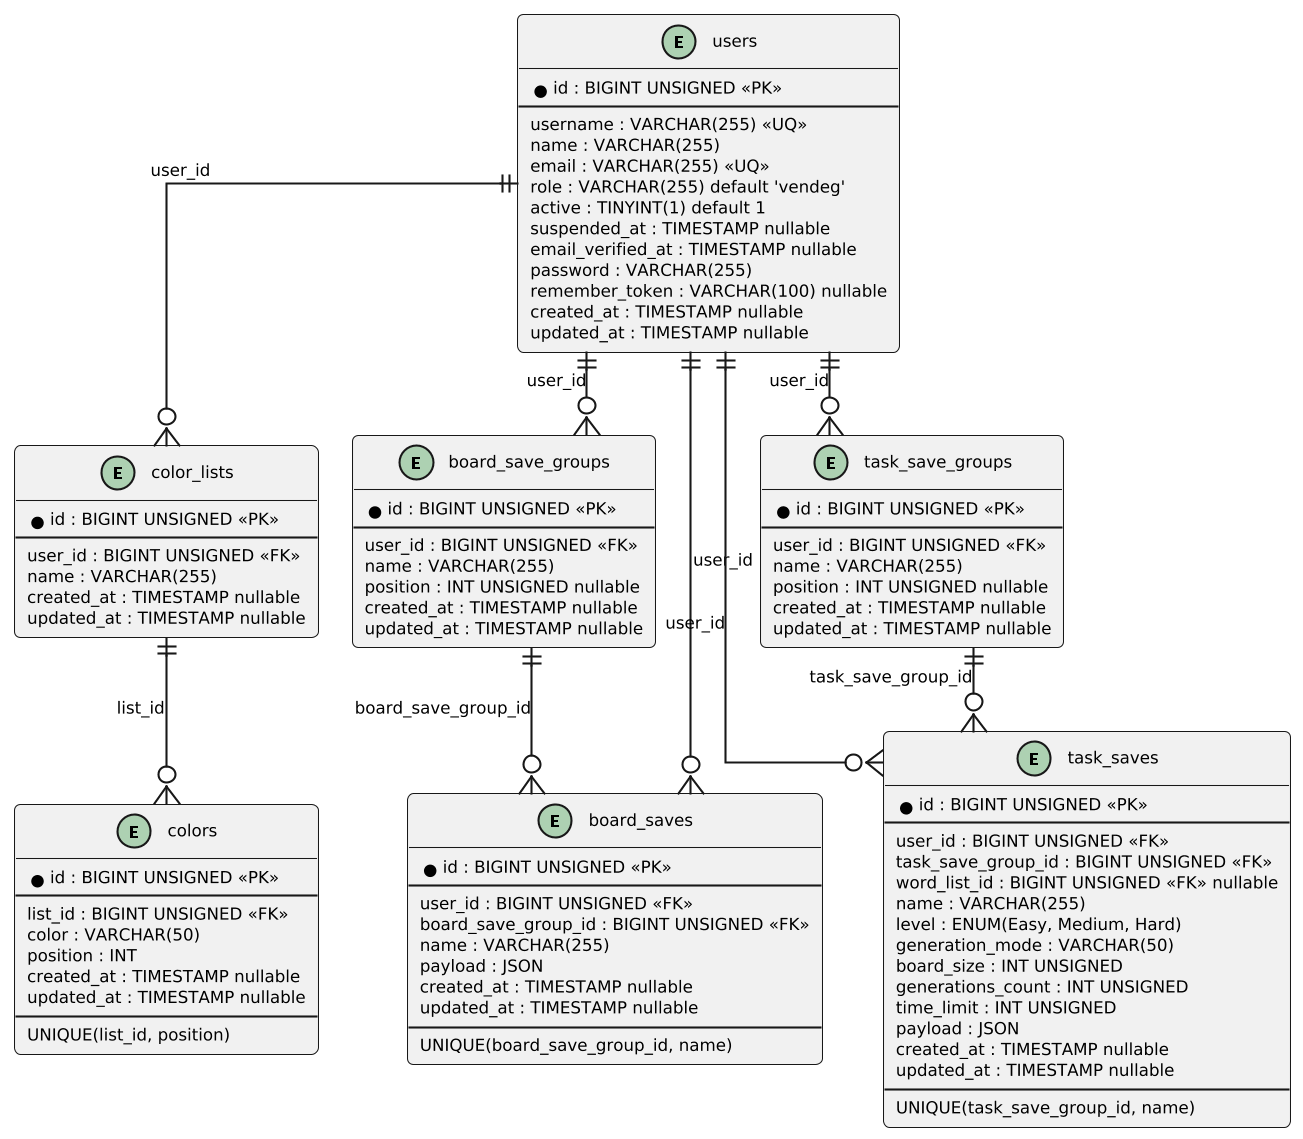
\includegraphics[width=0.96\textwidth]{uml_not_words.png}
\caption{UML diagram a relációs modell: colors, boards, tasks adatszerkezetekhez}
\end{figure}

\begin{figure}[htbp]
\centering
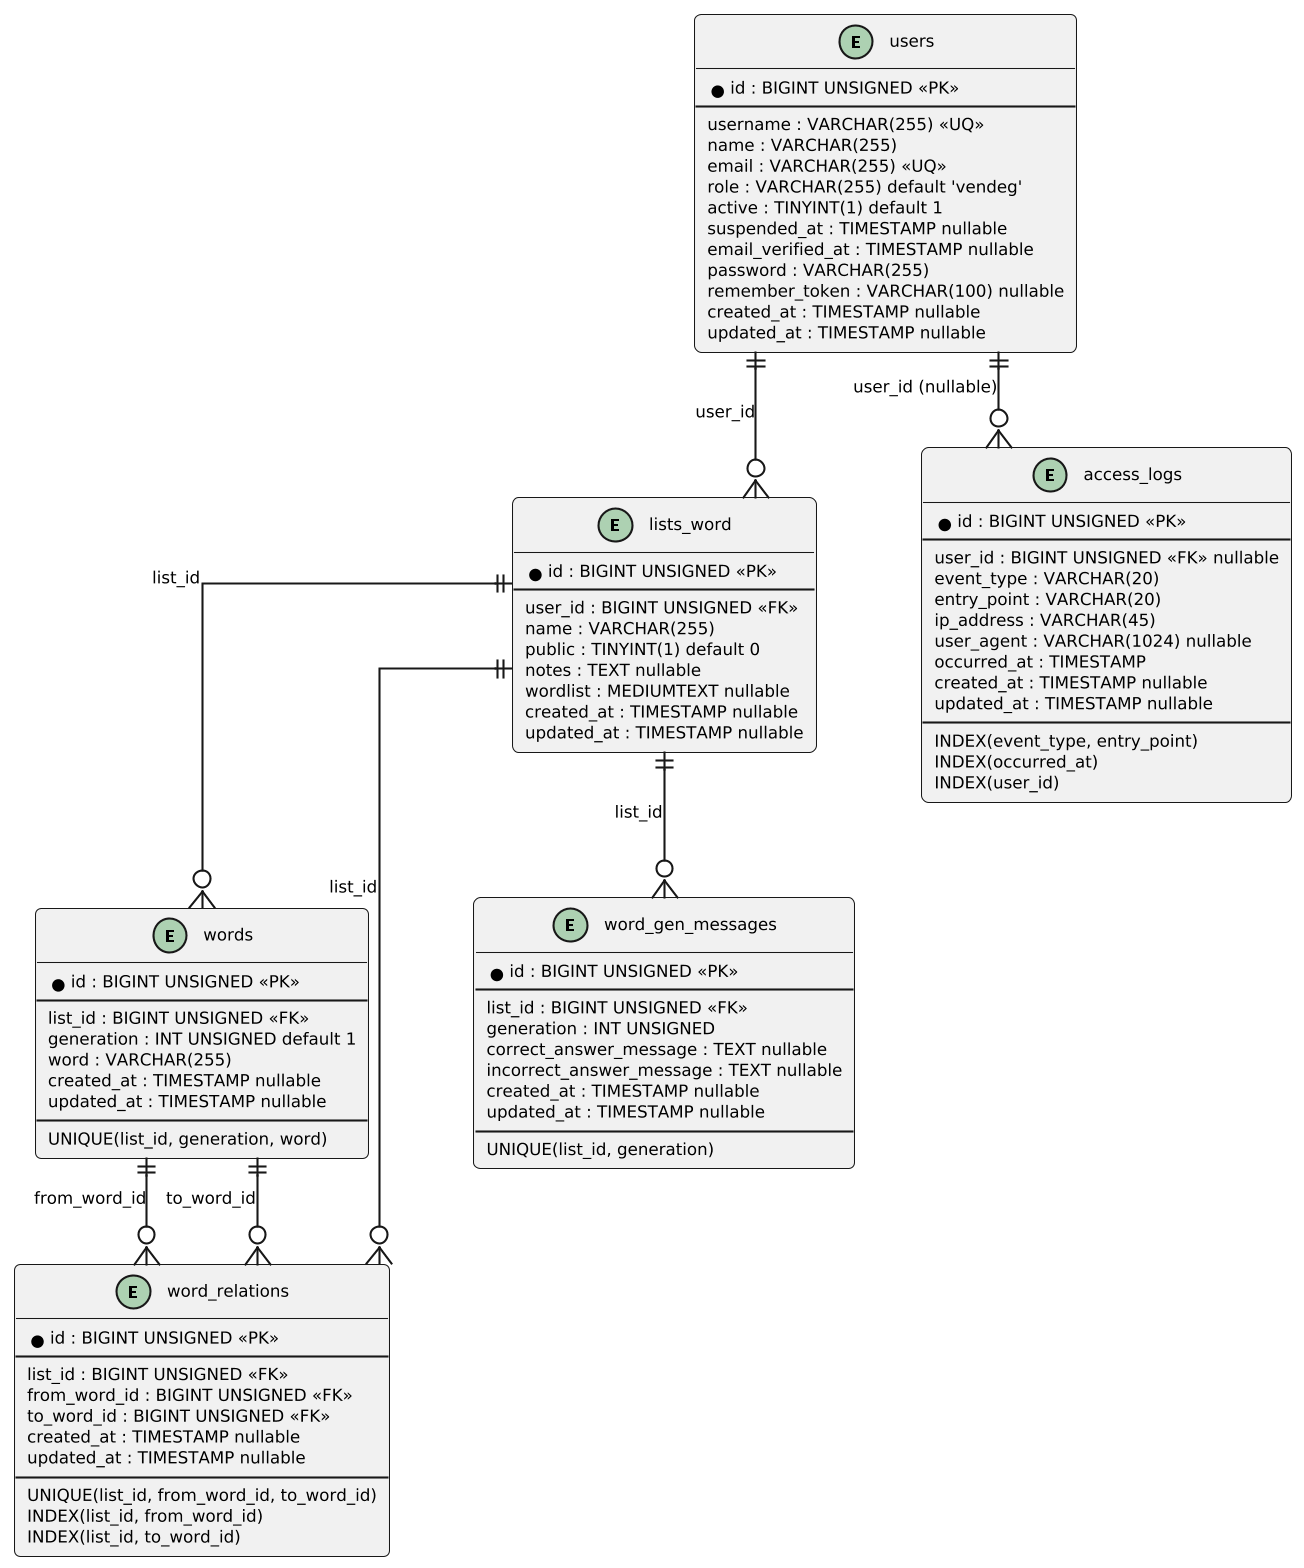
\includegraphics[width=0.96\textwidth]{uml_words.png}
\caption{UML diagram a relációs modell: words, access\_log adatszerkezetekhez}
\end{figure}

\chapter{Saját szoftver megvalósítása (Cellauto)}

\section{A backend implementáció}

A backend réteg feladata, hogy egységes API-felületet biztosítson az adminisztrációs és a felhasználói kliens számára. A megvalósítás Laravel 12 keretrendszerben, PHP 8.2 környezetben történt, ahol a routing, a middleware-kezelés, az autentikáció és az adatbázis-műveletek jól elkülönített felelősségi körök mentén működnek.

Az API végpontok kontrolleralapú szervezésben találhatók meg, a védett műveletek pedig Sanctum tokenes hitelesítéssel érhetők el. A \texttt{auth:sanctum} middleware biztosítja, hogy csak azonosított felhasználó végezhessen műveletet, míg az adminisztrációs végpontoknál az \texttt{admin} jogosultsági ellenőrzés korlátozza a hozzáférést.

A backend központi szerepe az adatintegritás és a konzisztencia fenntartása. Az adatmodellben alkalmazott idegen kulcsok, kompozit egyedi kulcsok és tulajdonosi ellenőrzések garantálják, hogy a szólisták, színlisták, valamint a mentési csoportok és mentések műveletei ne vezessenek inkonzisztens állapotokhoz.

\subsection{API és üzleti logika}
Az üzleti szabályok szerveroldalon érvényesülnek: a kliens csak a megengedett adatokat tudja módosítani, a validáció és a jogosultsági ellenőrzés minden kritikus műveletnél kötelező. Ez a megközelítés azért fontos, mert az admin és a publikus felület különböző hozzáférési modellel dolgozik, de ugyanarra az adatbázisra épül.

\subsection{Biztonság és naplózhatóság}
A hitelesítésen túl a rendszer kezeli az inaktív/felfüggesztett felhasználók hozzáférését is, továbbá naplózza a fontosabb hozzáférési eseményeket. Ennek gyakorlati haszna, hogy incidens vagy hibás működés esetén az eseménylánc visszakövethető, ami támogatja a stabil üzemeltetést és az auditálhatóságot.

\section{Az Admin felület (\texttt{admin})}

Az admin felület a rendszer üzemeltetésének és szakmai karbantartásának központi eszköze. A bal oldali menüre épülő moduláris felépítés miatt az adminisztrátor jól elkülönített funkcionális területeken tud dolgozni: felhasználókezelés, szólista- és színlista-szerkesztés, vizsgaeredmények elemzése, valamint hozzáférési naplók ellenőrzése.

A felület tervezési célja a gyors és biztonságos adminisztráció támogatása. A táblázatos nézetek, keresési lehetőségek, visszajelző üzenetek és megerősítő lépések együtt csökkentik a hibázási kockázatot, különösen nagyobb adatmennyiség esetén.

\subsection{Felhasználókezelés}
A felhasználókezelés az admin felület egyik alapmodulja, amely a fiókok teljes életciklusának kezelését támogatja. A modul célja, hogy az adminisztrátor egy központi felületen keresztül végezhesse a létrehozási, módosítási, aktiválási és törlési műveleteket, miközben a rendszer megőrzi a jogosultsági és adatkonzisztencia-korlátokat.

A funkció kizárólag admin szerepkörrel érhető el. Nem admin felhasználó esetén a rendszer nem engedélyezi a műveletek végrehajtását, így csökken a jogosulatlan adatváltoztatás kockázata.

\paragraph{Támogatott szerepkörök és hozzáférés.}
A felhasználók a rendszerben szerepkörhöz kötött jogosultságokat kapnak (például vendég, diák, tanár, admin). A beállított szerepkör meghatározza, hogy a felhasználó mely rendszerfunkciókat látja, és milyen műveleteket hajthat végre.

\paragraph{Alapműveletek.}
A modul a következő fő műveleteket biztosítja:
\begin{itemize}
  \item új felhasználó létrehozása kötelező adatokkal (felhasználónév, név, email, jelszó, szerepkör);
  \item meglévő rekord szerkesztése, beleértve a szerepkör módosítását;
  \item felhasználó felfüggesztése és visszaaktiválása törlés nélkül;
  \item végleges törlés védelmi szabályok mellett (például saját fiók vagy admin fiók törlésének korlátozása).
\end{itemize}

\paragraph{Keresés és áttekinthetőség.}
A listanézet szöveges keresőt biztosít, amely azonosító, név, felhasználónév, email és szerepkör mezők alapján szűr. Ez nagyobb felhasználószám esetén is gyors és célzott adminisztrációt tesz lehetővé.

\paragraph{Visszajelzés és működési biztonság.}
A felület minden művelet után egyértelmű sikeres vagy hibás állapotüzenetet jelenít meg. A kockázatos lépésekhez megerősítő párbeszédablak tartozik, ami támogatja a tudatos, kontrollált módosítást és csökkenti a véletlen hibák esélyét.

\begin{figure}[htbp]
\centering
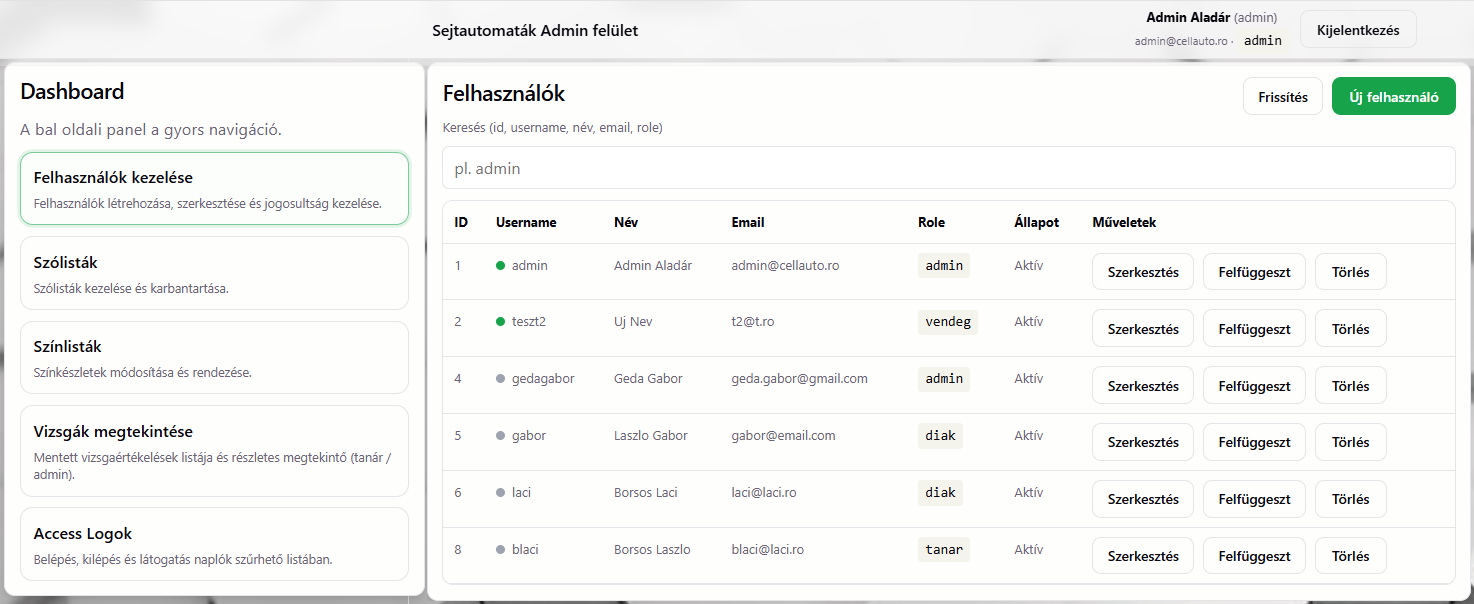
\includegraphics[width=0.92\textwidth]{Admin - a felhasznalok kezelese.png}
\caption{Admin felület: felhasználók kezelése}
\end{figure}

\subsection{Szólisták kezelése}
A szólisták kezelése az admin felület egyik központi funkciója, mivel ez biztosítja a feladatok nyelvi tartalmának előállítását és folyamatos karbantartását. A modul célja, hogy az adminisztrátor és a tanári szerepkör gyorsan, mégis következetesen tudja felépíteni azt a szókészletet, amelyre a gyakorló és vizsgafeladatok épülnek.

A szólista nem egyszerű felsorolás, hanem a feladatgenerálás alapadata. A megfelelően szerkesztett lista és a hozzá tartozó relációk közvetlenül befolyásolják a létrejövő mondatok minőségét, a feladatok nehézségét és a kiértékelés szakmai értelmezhetőségét.

\paragraph{Fő kezelési műveletek.}
A modulban végrehajtható legfontosabb műveletek:
\begin{itemize}
  \item új szólista létrehozása és alapadatainak megadása;
  \item meglévő listaelemek szerkesztése, javítása és bővítése;
  \item szavak közötti relációk definiálása a mondatgenerálás logikai alapjaként;
  \item a generált mondatok és kapcsolatok szakmai ellenőrzése;
  \item folyamatos karbantartás és finomhangolás a gyakorlati tapasztalatok alapján.
\end{itemize}

\paragraph{Kapcsolat a feladatgenerálással.}
A rendszer által használt mondatstruktúra közvetlenül a szólistákból és relációikból épül fel. Ennek következtében a szólistakezelés minősége meghatározza, hogy a tanuló mennyire releváns, pedagógiailag hasznos és értelmezhető feladatokat kap.

\paragraph{Használhatósági és minőségbiztosítási szempontok.}
A felület hagyományos és vizuális szerkesztési módot is támogat, ami segíti a komplex kapcsolatok áttekinthető kezelését. A gyors adatbevitel, a rendezett vizuális struktúra, valamint a kapcsolatok és mondatok együttes megjelenítése csökkenti a szerkesztési hibák számát.

A szólisták karbantartása minőségbiztosítási feladat is: pontatlan vagy hiányos lista esetén hibás mondatok keletkezhetnek, ami félrevezető feladatokat eredményezhet. Ezért a modulban végzett munka nemcsak technikai, hanem módszertani szempontból is kritikus.

\begin{figure}[htbp]
\centering
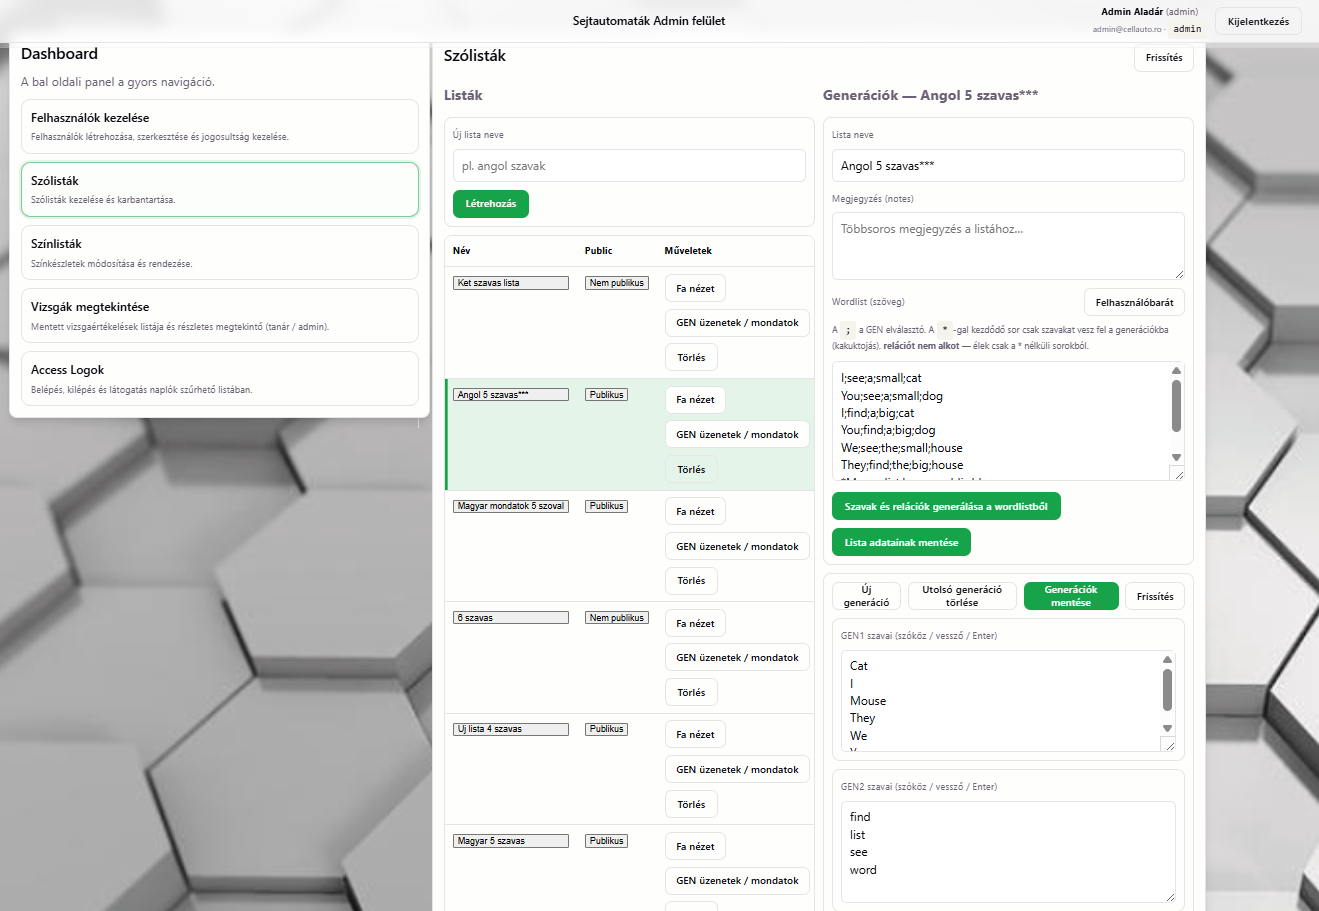
\includegraphics[width=0.92\textwidth]{Admin - a szolista szerkesztese.png}
\caption{Admin felület: szólista szerkesztése}
\end{figure}

\begin{figure}[htbp]
\centering
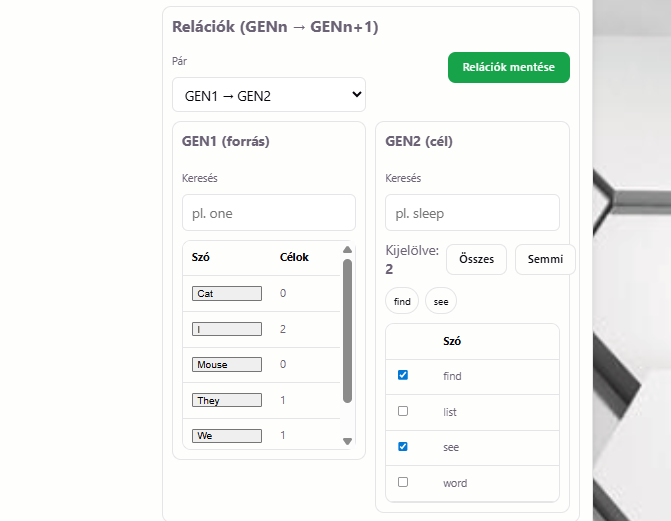
\includegraphics[width=0.92\textwidth]{Admin - a szolista relacioinak megadasa hagyomanyos modon.png}
\caption{Admin felület: szólista-relációk megadása hagyományos módon}
\end{figure}

\begin{figure}[htbp]
\centering
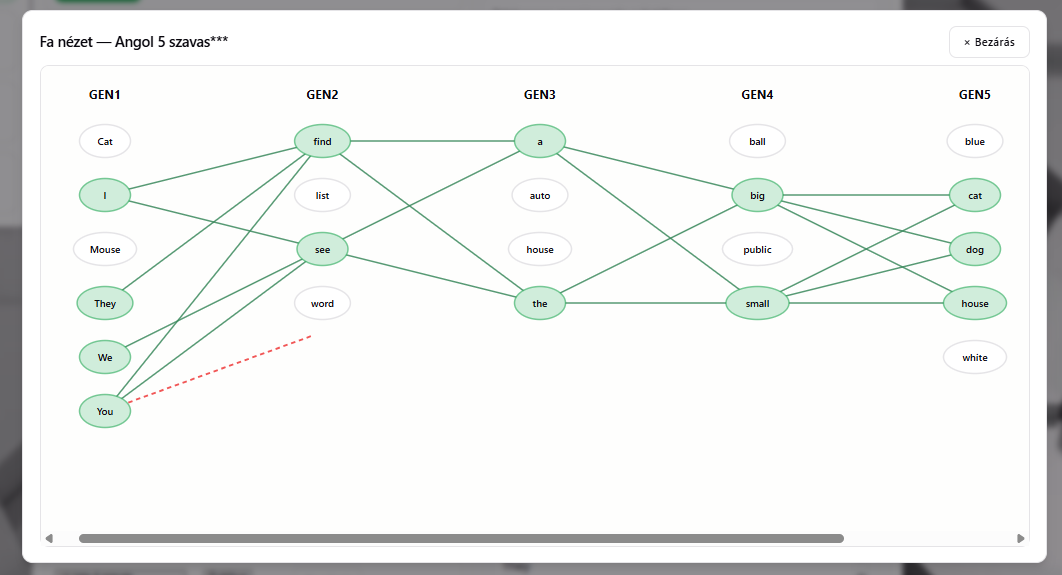
\includegraphics[width=0.92\textwidth]{Admin - a szolista relaciok vizualis nezete - szerkesztese egerrel.png}
\caption{Admin felület: szólista-relációk vizuális szerkesztése}
\end{figure}

\begin{figure}[htbp]
\centering
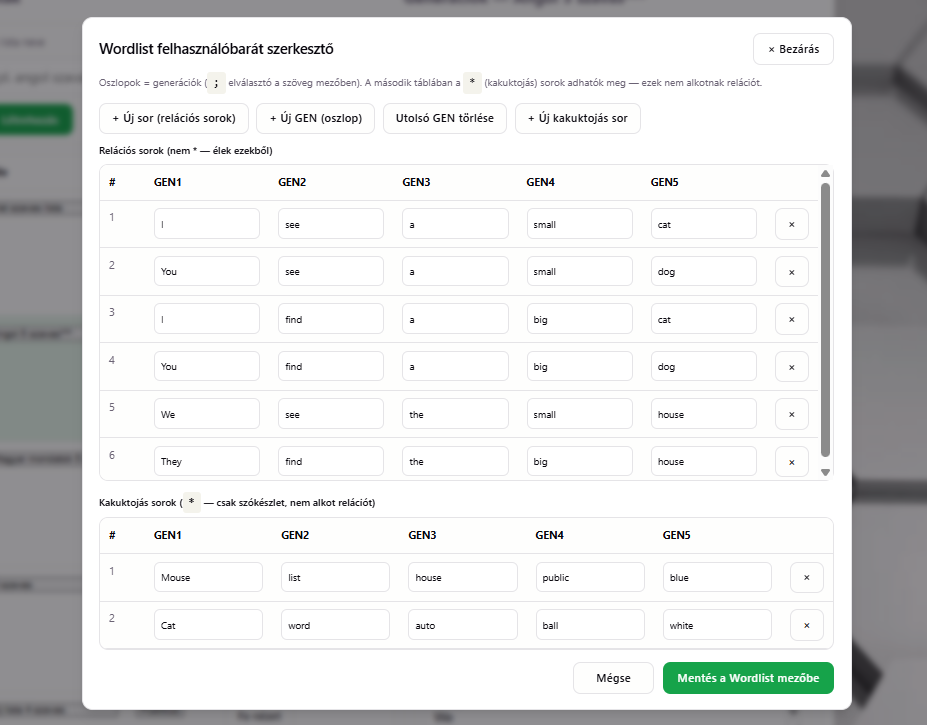
\includegraphics[width=0.92\textwidth]{Admin - a szolista felhasznalobarat modon torteno relaciok es szavak kezelese mondatonkent.png}
\caption{Admin felület: felhasználóbarát szó- és relációkezelés mondatonként}
\end{figure}

\begin{figure}[htbp]
\centering
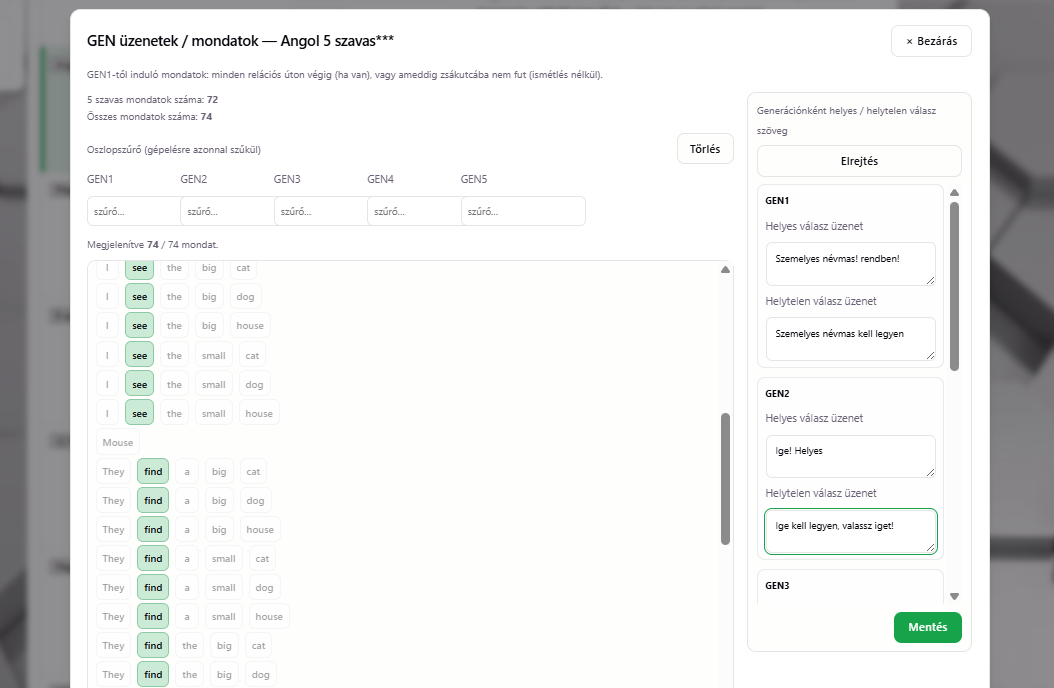
\includegraphics[width=0.92\textwidth]{Admin - a szolista generacios uzeneteinek kezelese es mondatok.png}
\caption{Admin felület: generációs üzenetek és mondatok kezelése}
\end{figure}
\FloatBarrier

\subsection{Színlisták kezelése}
A színlisták kezelése az admin felület olyan funkciója, amely a vizuális kategorizálást és a feladatok áttekinthetőségét támogatja. A modul célja, hogy a szakmai felhasználó (admin és tanár) egységes, pedagógiailag értelmezhető színstruktúrát tudjon kialakítani és karbantartani.

A színlisták a rendszerben nem pusztán megjelenítési elemek. A vizuális jelölések segítik az információ gyors feldolgozását, a mintázatok felismerését és a feladatmegoldás támogatását. Egy következetesen felépített színrendszer különösen összetettebb táblák és relációk esetén csökkenti a kognitív terhelést.

\paragraph{Fő kezelési műveletek.}
A modul a következő fő műveleteket biztosítja:
\begin{itemize}
  \item új színlista létrehozása a szükséges alapadatokkal;
  \item meglévő elemek szerkesztése, színek finomhangolása, elnevezések pontosítása;
  \item rendezés és struktúra-kezelés a kategóriák logikus csoportosításához;
  \item karbantartás, az elavult vagy nem használt elemek felülvizsgálatával.
\end{itemize}

\paragraph{Kapcsolat a felhasználói élménnyel.}
A színlisták közvetlenül befolyásolják a felület értelmezhetőségét. Ha a színek következetesen vannak használva, a tanuló és az oktató gyorsabban azonosítja a fontos elemeket, így a rendszer kezelése intuitívabbá válik.

\paragraph{Használhatósági és minőségi szempontok.}
A színkezelés során kiemelt szempont:
\begin{itemize}
  \item a konzisztencia (azonos jelentéshez azonos szín);
  \item az olvashatóság (megfelelő kontraszt és vizuális elkülöníthetőség);
  \item a karbantarthatóság (későbbi bővítés egyszerűsége).
\end{itemize}

Ezek együtt biztosítják, hogy a vizuális jelölések hosszú távon is támogassák a rendszer pedagógiai céljait.

\begin{figure}[htbp]
\centering
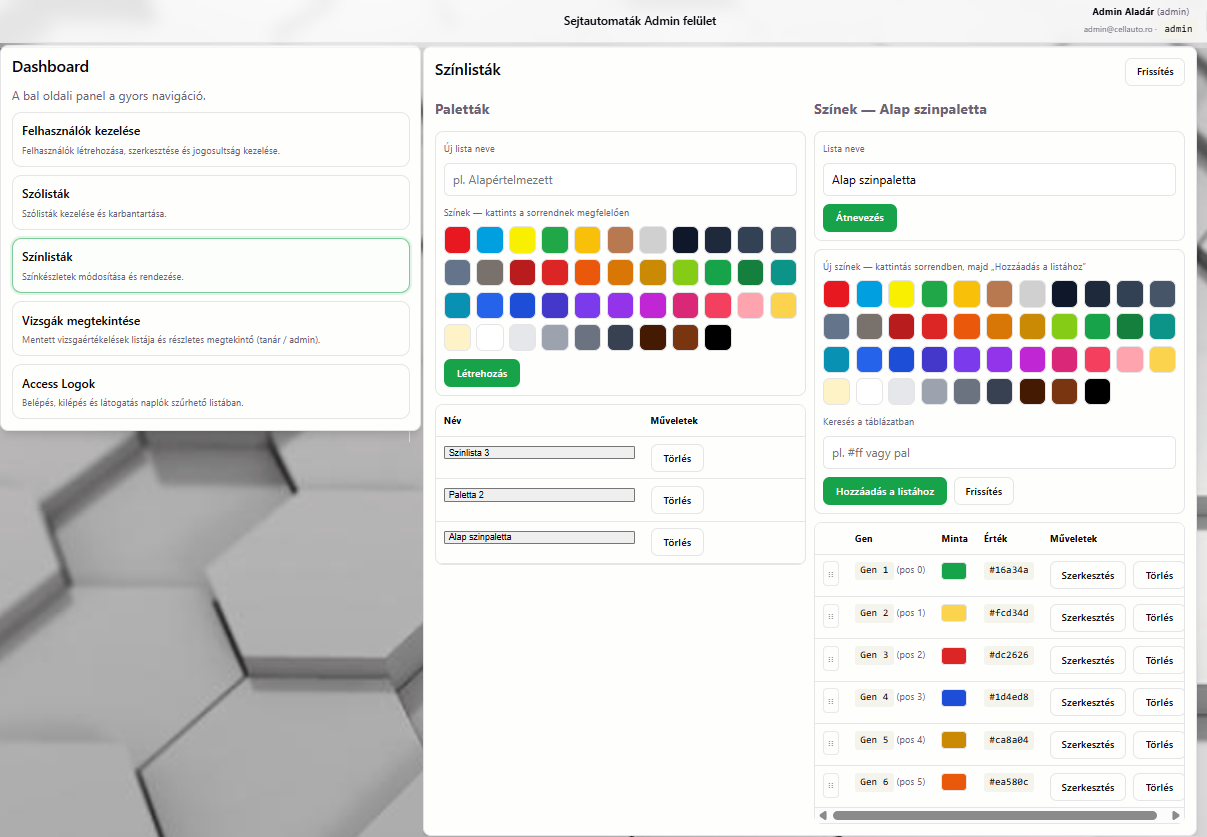
\includegraphics[width=0.92\textwidth]{Admin - a szinlista szerkeszto.png}
\caption{Admin felület: színlista szerkesztése}
\end{figure}
\FloatBarrier

\subsection{Vizsgák megtekintése}
A ``Vizsgák megtekintése'' modul az admin felületen a teljesítményadatok ellenőrzését és elemzését szolgálja. A funkció célja, hogy az oktató vagy admin gyorsan át tudja tekinteni a mentett vizsgaeredményeket, majd egy kiválasztott sor részleteit részletesen is megvizsgálhassa.

A vizsgamodul összeköti az értékelési folyamatot az adminisztratív döntéstámogatással. Segítségével nemcsak az látható, hogy egy felhasználó mikor és milyen eredményt ért el, hanem az is, hogy a hibák milyen jellegűek voltak (például cella- vagy mondatszintű eltérések).

\paragraph{Listanézet és szűrés.}
A modul első szintje egy táblázatos listanézet, amely a legfontosabb adatokat jeleníti meg: vizsga dátuma, tanuló adatai, kapcsolódó feladat, cellaeredmény százalékos mutatója, mondateredmény százalékos mutatója, megjegyzés.

A lista szűrhető dátumtartomány, felhasználó, feladatnév és megjegyzés alapján. Ez különösen hasznos nagy adatmennyiségnél, amikor célzottan kell visszakeresni egy adott időszakot vagy felhasználót.

\paragraph{Részletes nézet (modális ablak).}
Egy sor kiválasztásakor a rendszer modális ablakban jeleníti meg a részletes vizsgaadatokat. Itt az admin láthatja az azonosító és időbélyeg információkat, az összegző teljesítménymutatókat, a cellák és mondatok számszerű bontását, a megjegyzést, valamint a mondateredmény szöveges részleteit. A modális megjelenítés előnye, hogy a felhasználó a lista kontextusának elhagyása nélkül tud részleteket elemezni.

\paragraph{Használhatósági és pedagógiai jelentőség.}
A modul kialakítása támogatja a gyakorlati használatot: az adatok lapozott formában jelennek meg, a táblázat és a részletes nézet gyors átjárást biztosít a makro- és mikroszintű elemzés között, hosszabb tartalom esetén pedig a modális ablak görgethető marad.

A vizsgák áttekintése nemcsak technikai riportálás, hanem pedagógiai visszacsatolás is. A részletes adatok alapján az oktató pontosabban azonosíthatja a tipikus hibamintákat, így célzottabb fejlesztő feladatokat tud adni.

\begin{figure}[!htbp]
\centering
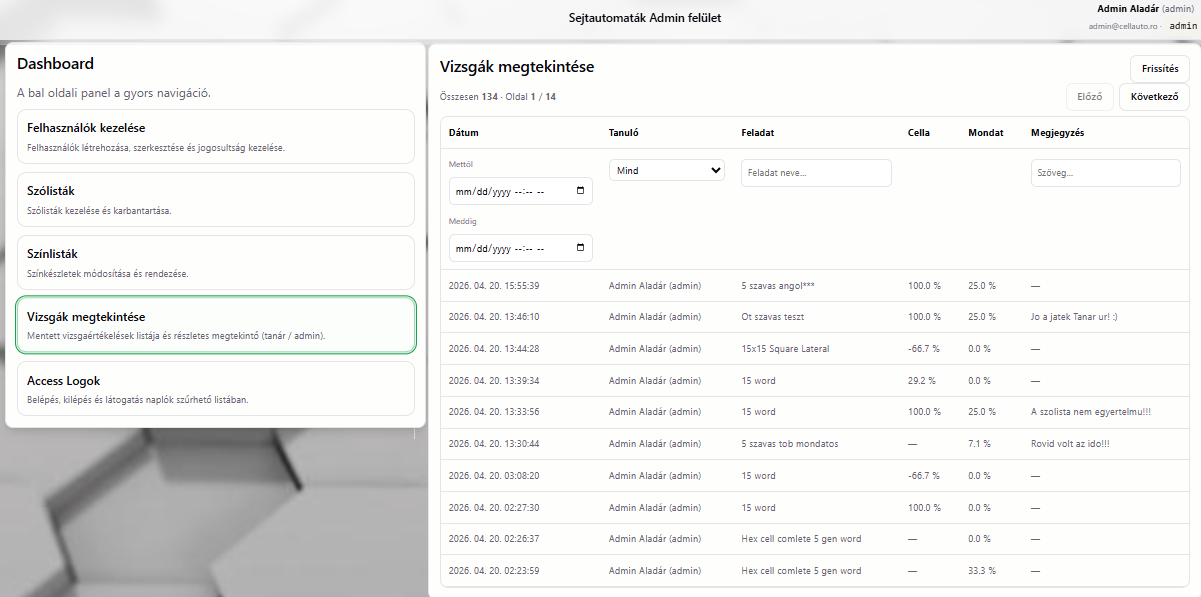
\includegraphics[width=0.84\textwidth]{Admin - a Vizsgak kiertekelese - lista.png}
\caption{Admin felület: vizsgaeredmények listája}
\end{figure}

\begin{figure}[!htbp]
\centering
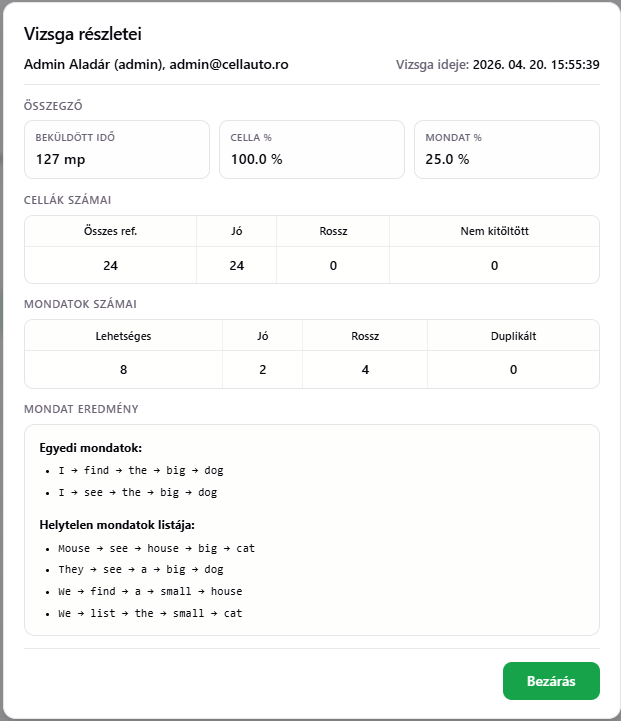
\includegraphics[width=0.68\textwidth]{Admin - a Vizsgak kiertekelesenek reszletei.png}
\caption{Admin felület: vizsgaeredmény részletes nézete}
\end{figure}
\FloatBarrier

\subsection{Naplók}
Az Access Logok modul az admin felület auditálási és ellenőrzési funkcióját biztosítja. Célja, hogy a rendszerhasználathoz kapcsolódó események (például belépések, kilépések, aktivitási nyomok) visszakereshetők és áttekinthetők legyenek.

A naplózási funkció a biztonság és az üzemeltetés szempontjából kiemelten fontos. Segítségével az adminisztrátor képet kap arról, hogy ki, mikor és milyen körülmények között használta a rendszert.

\paragraph{Fő funkciók.}
\begin{itemize}
  \item Naplóbejegyzések listázása időrendi sorrendben;
  \item szűrés és keresés felhasználó, időszak vagy eseménytípus szerint;
  \item áttekinthető, táblázatos megjelenítés;
  \item visszakövethetőség problémák vagy rendellenes használat esetén.
\end{itemize}

\paragraph{Üzemeltetési és biztonsági jelentőség.}
Az Access Logok modul segít azonosítani a jogosulatlan vagy gyanús hozzáférési mintákat, támogatja a hibakeresést és incidensvizsgálatot, alapot ad a belső auditfolyamatokhoz, valamint növeli az üzemeltetés átláthatóságát és elszámoltathatóságát.

\paragraph{Pedagógiai környezetben betöltött szerep.}
Oktatási környezetben különösen fontos a felhasználói tevékenységek ellenőrizhetősége, mivel a rendszer vizsgaeredményeket és tanulói adatokat is kezel. A naplóadatok ezért nemcsak technikai, hanem adatvédelmi és szervezeti szempontból is relevánsak.

\begin{figure}[htbp]
\centering

\includegraphics[width=0.92\textwidth]{Admin - Naplozas.png}
\caption{Admin felület: naplózási nézet}
\end{figure}
\FloatBarrier

\section{A felhasználói felület (\texttt{www})}

A felhasználói felület célja, hogy a sejtautomata-alapú tanulási folyamatot egyszerre tegye szemléletessé és jól gyakorolhatóvá. A rendszer vendég módban is használható, ugyanakkor bejelentkezett állapotban teljes funkcionalitást nyújt: mentések, szólistaalapú kitöltés, gyakorlás és vizsga.

A Cellauto webalkalmazás a sejtautomaták működésének szimulációjára épül, és oktatási, valamint kutatási célra egyaránt használható. A felület kialakításának egyik fő erőssége, hogy játékos formában támogatja a logikus gondolkodás és a kreativitás fejlesztését, miközben szólistás és mondatalkotási elemekkel a nyelvhelyesség és a nyelvtanulás gyakorlását is segíti.

\subsection{Homokozó és bejelentkezett használat}
A felület bejelentkezés nélkül is kipróbálható egy alap homokozó módban, amely lokálisan fut, és adatbázis-művelet nélkül teszi lehetővé a sejtautomata működésének szabad tesztelését. Ez a mód különösen hasznos első megismeréshez, kísérletezéshez és szemléltetéshez.

Bejelentkezett állapotban a rendszer a backend szolgáltatásait is elérhetővé teszi: a felhasználó elmentheti saját munkáját (sejtszerkezetét), gyakorolhat tanári feladatokon, illetve vizsgát is teljesíthet.

\begin{figure}[htbp]
\centering
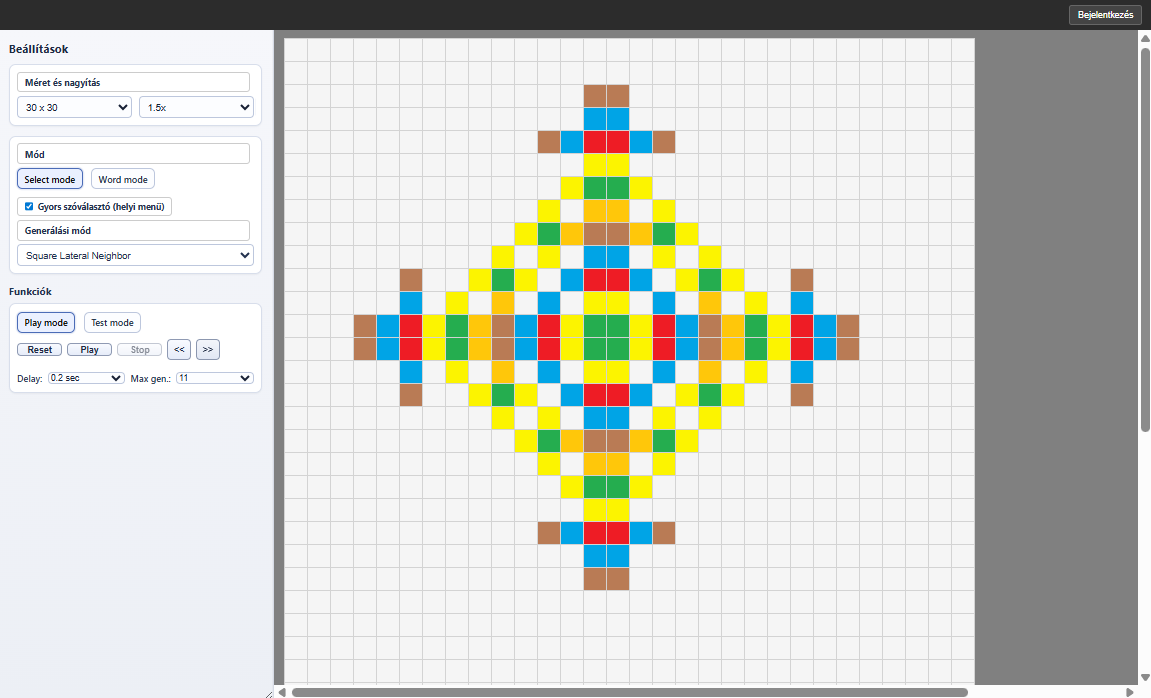
\includegraphics[width=0.88\textwidth]{Sejtauomatta felulete - bejelentkezes nelkul.png}
\caption{Felhasználói felület: homokozó mód bejelentkezés nélkül}
\end{figure}

\begin{figure}[H]
\centering
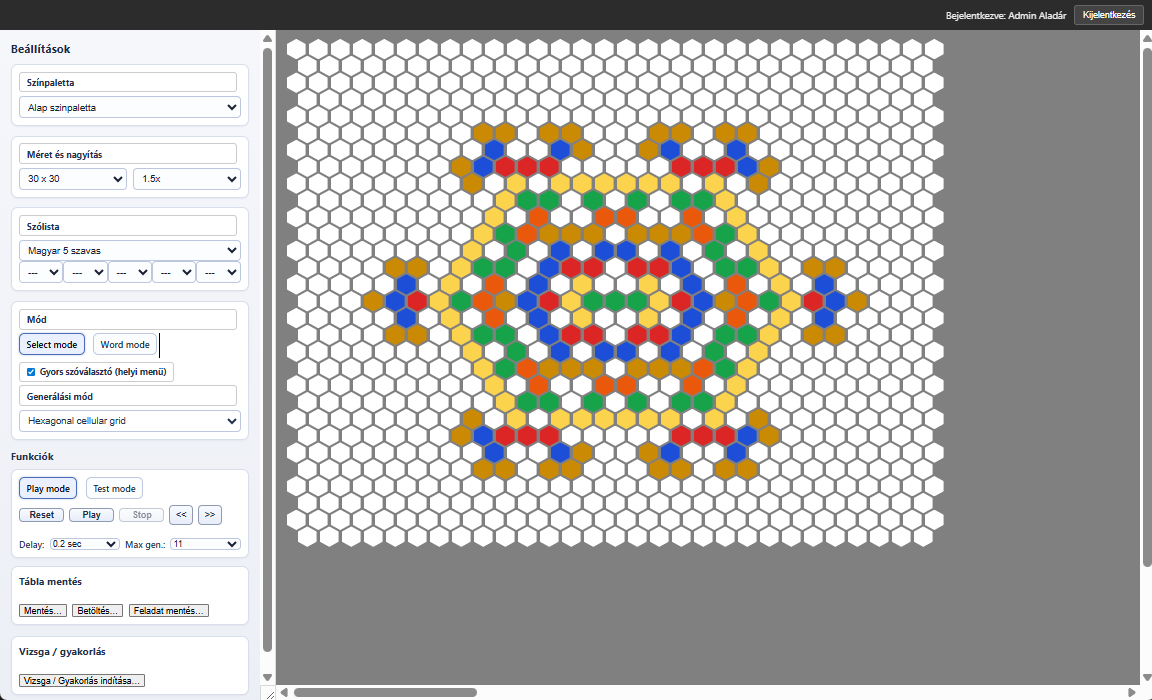
\includegraphics[width=0.88\textwidth]{Sejtautomatta bejelentkezessel - a homokozoval.png}
\caption{Felhasználói felület: bejelentkezett nézet}
\end{figure}

\subsection{Feladatok, szerepkörök és mentések}
A rendszer több szerepkörös működést támogat (admin, tanár, diák, vendég), ezért a felhasználó által elérhető funkciók a szerepkörtől függenek. A tanári szerepkörben feladatok állíthatók össze a diákok számára, amelyeket a diák gyakorolhat vagy vizsgahelyzetben oldhat meg.

A tanári feladatkészítés több formában történhet:
\begin{itemize}
  \item tisztán sejtautomata-alapú feladat, ahol a tanár kiinduló pozíciókat ad meg, és a diáknak meghatározott generációig kell folytatnia;
  \item szólistával támogatott feladat, ahol a sejtes logika mellett nyelvileg helyes mondatokat kell kirakni;
  \item vegyes feladat, ahol a sejtautomata rész sikeres megoldása után lehet továbblépni a szó- és mondatkiegészítésre.
\end{itemize}

A felhasználó a szólisták elemeit közvetlenül beillesztheti a cellákba, majd a létrehozott állapotot elmentheti. A mentési funkció támogatja a hosszabb tanulási folyamatot, mert a korábbi állapotok később visszatölthetők és összehasonlíthatók.

\begin{figure}[htbp]
\centering
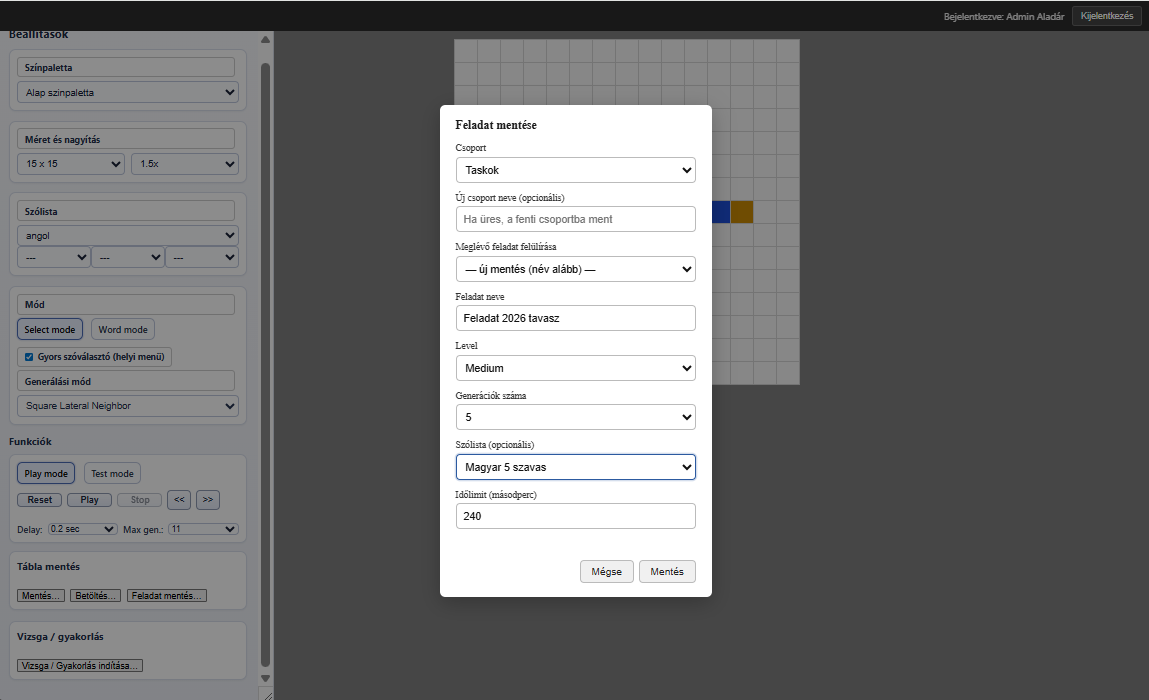
\includegraphics[width=0.88\textwidth]{Sejtautomatta - Feladat mentese - keszitese a vizsgahoz.png}
\caption{Felhasználói felület: feladat mentése vizsgához}
\end{figure}

\begin{figure}[htbp]
\centering
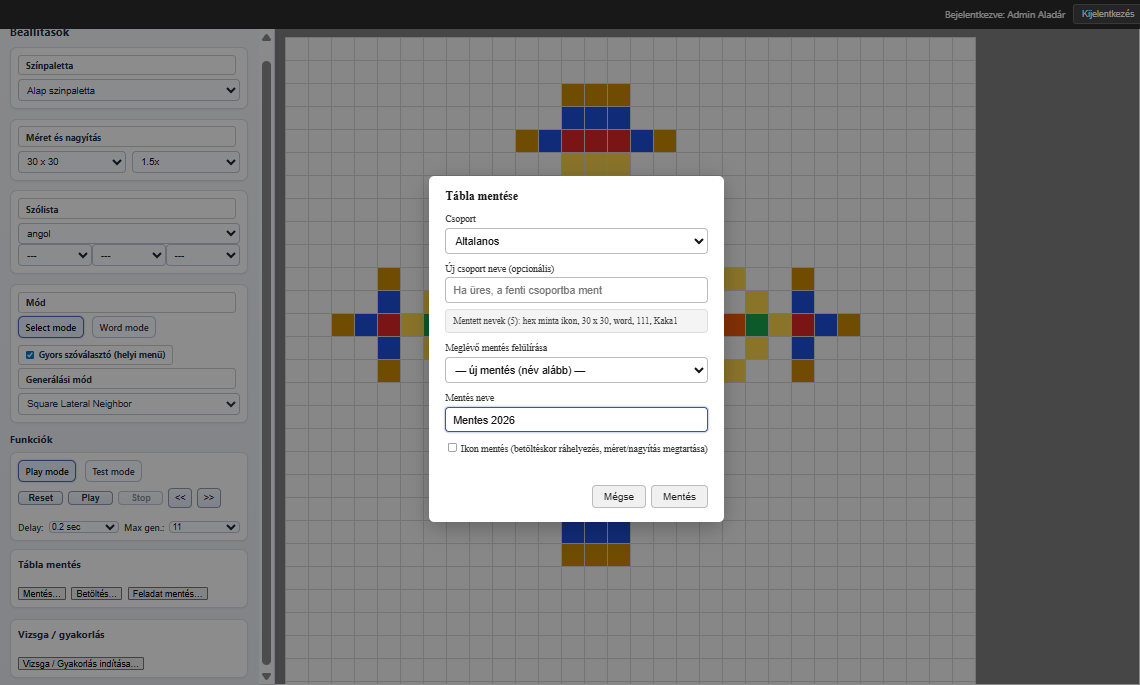
\includegraphics[width=0.88\textwidth]{Sejtautomatta Tabla allapot elmentese.png}
\caption{Felhasználói felület: táblaállapot mentése}
\end{figure}

\begin{figure}[htbp]
\centering
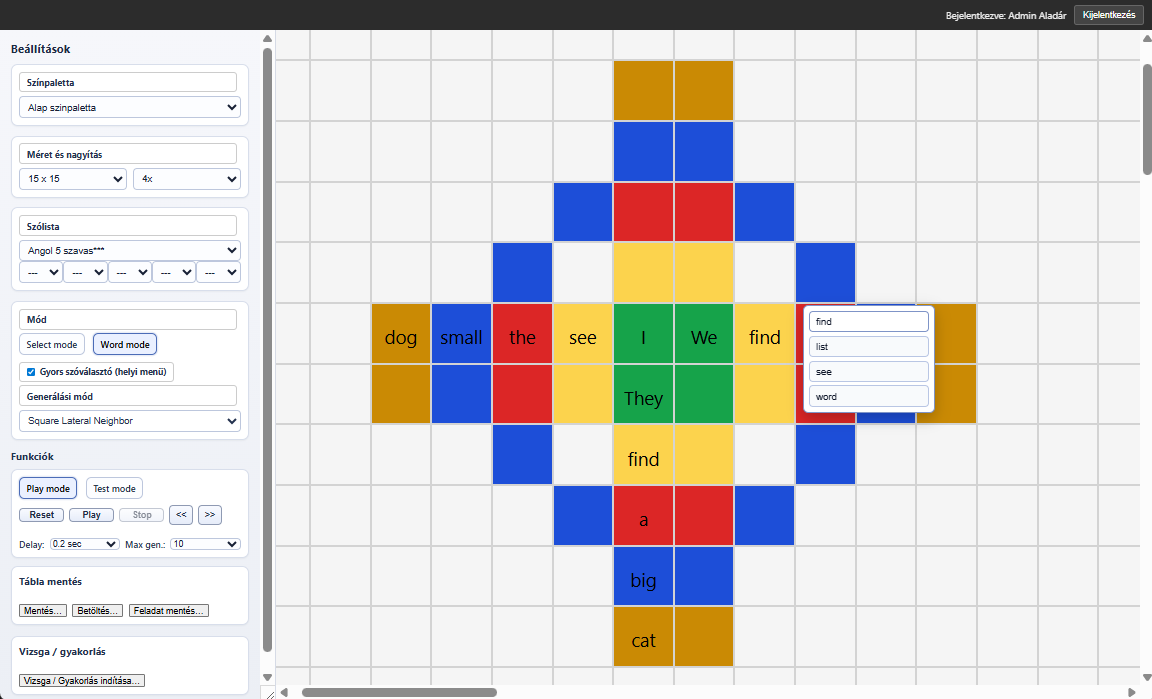
\includegraphics[width=0.88\textwidth]{Sejtautomatta - a szavak betetele a cellakba a szolistabol.png}
\caption{Felhasználói felület: szavak beillesztése a cellákba}
\end{figure}

\begin{figure}[htbp]
\centering
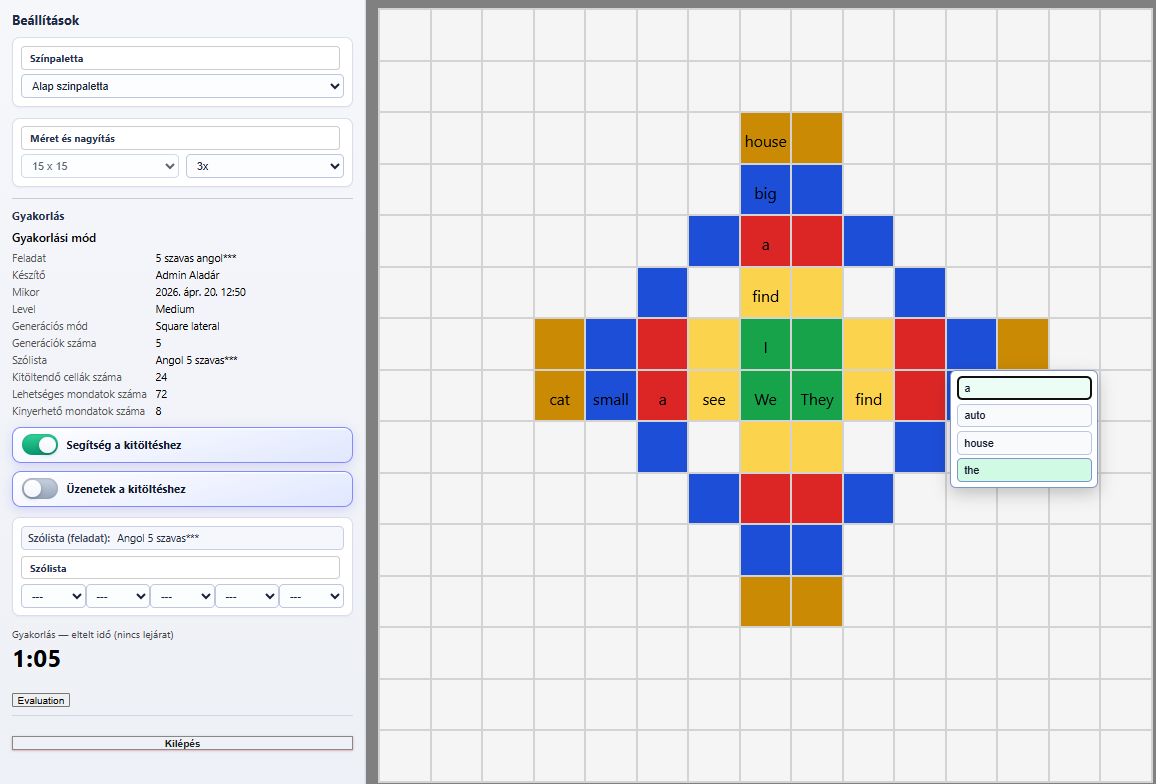
\includegraphics[width=0.88\textwidth]{Sejtautomatta - Gyakorlasi mod - Jo szavak mutatasa.png}
\caption{Felhasználói felület: gyakorlási mód visszajelzéssel}
\end{figure}

Vizsgamódban a rendszer időkerettel és automatikus kiértékeléssel működik. A beadott megoldás alapján a cellaszintű és mondatszintű eredmények is rögzítésre kerülnek, így a felhasználó részletes visszacsatolást kap a teljesítményéről.

Ha az időkorlát lejár, a rendszer automatikusan elvégzi a kiértékelést, de a diák korábban is kezdeményezheti azt. A vizsgaeredményhez kapcsolódva mentésre kerül a teljesítési idő is, amelyet a tanár később visszanézhet az admin felületen.

A vizsga végén a diák üzenetet is hagyhat a tanárnak (például ha a feladat vagy szólista nem egyértelmű). Ez a megjegyzés a kiértékeléshez csatolva tárolódik, így a tanár a teljesítményadatokkal együtt tudja értelmezni a visszajelzést.

\begin{figure}[htbp]
\centering
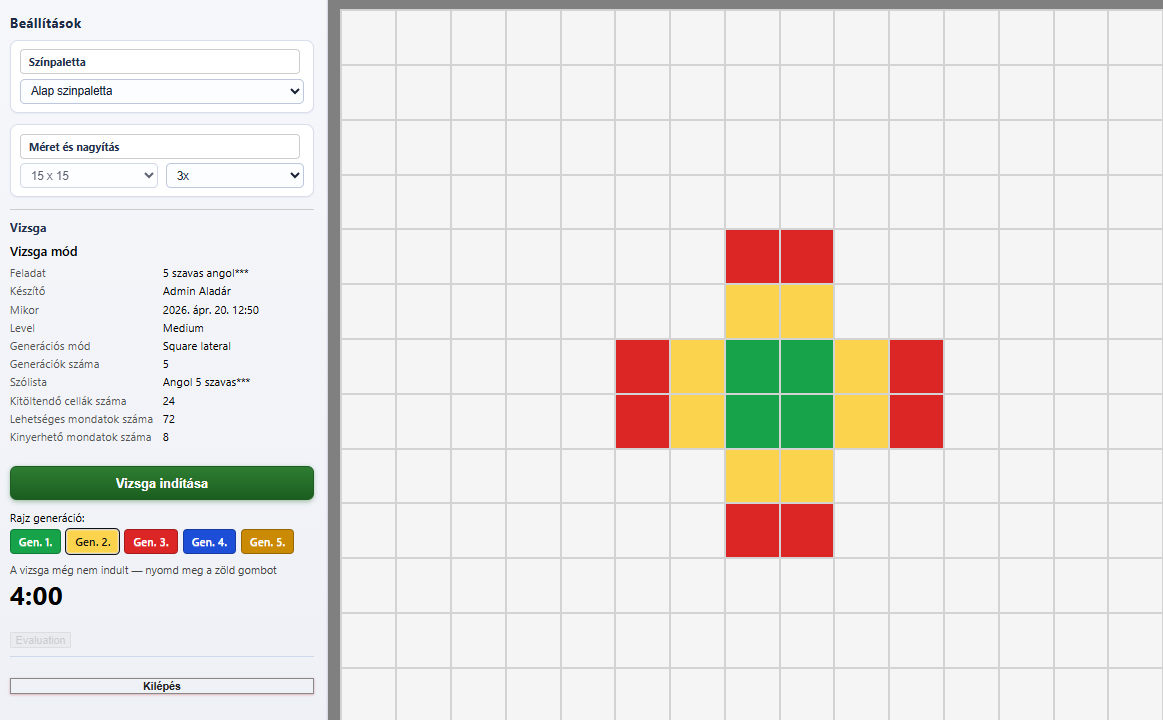
\includegraphics[width=0.88\textwidth]{Sejtautomatta - Vizsga - Cellak es Szavak.png}
\caption{Felhasználói felület: vizsgafelület}
\end{figure}

\begin{figure}[htbp]
\centering
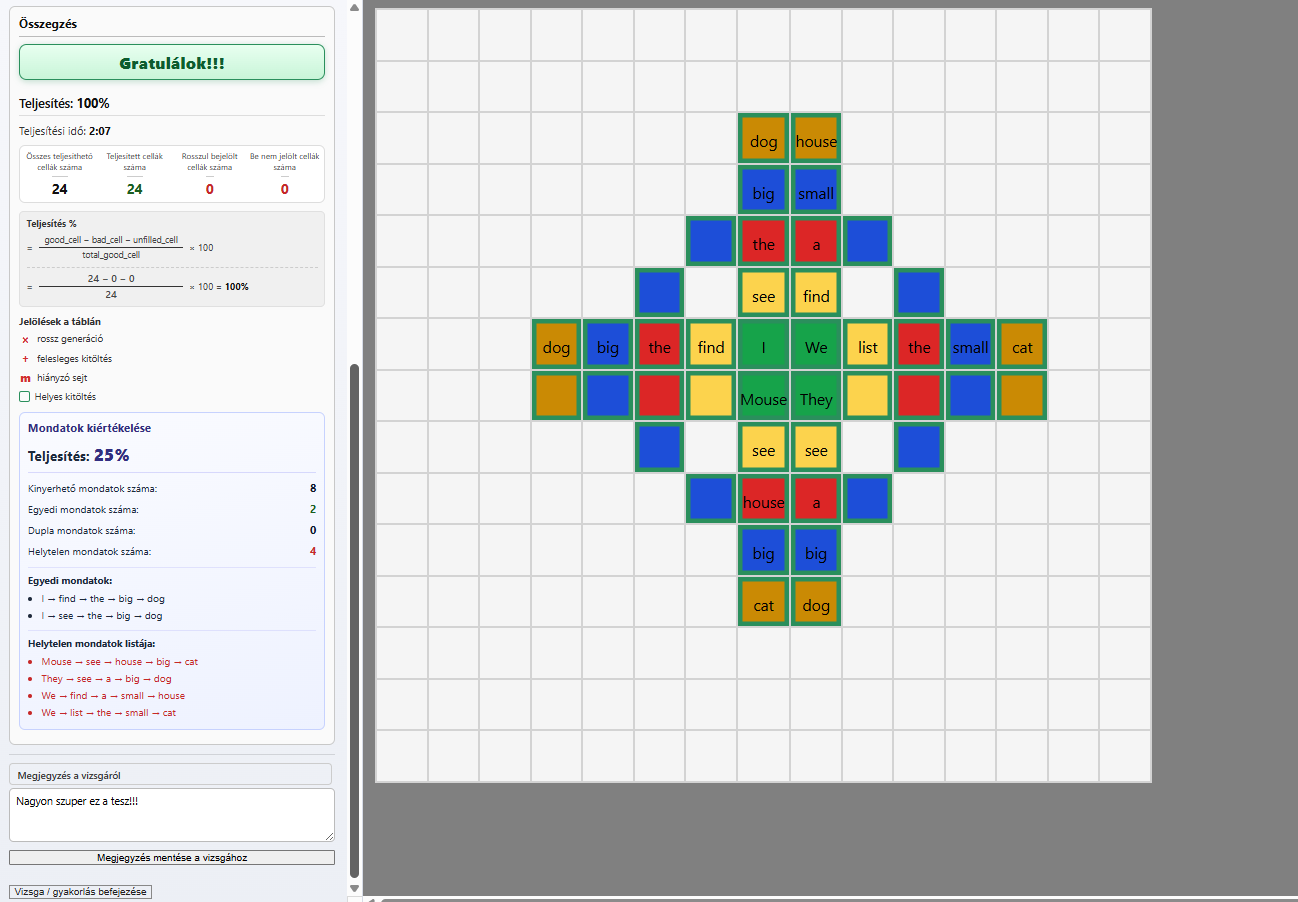
\includegraphics[width=0.88\textwidth]{Sejtautomatta - Vizsga kiertekeles.png}
\caption{Felhasználói felület: vizsga kiértékelése}
\end{figure}

\section{Életjáték (Game of Life)}
A rendszer egyik különleges eleme, hogy a generációs módok között elérhető a Conway-féle \emph{Game of Life} implementáció is. Ez a modul nem klasszikus értelemben vett gyakorló- vagy vizsgafeladatként jelenik meg, hanem szemléltető és kísérletező célú funkcióként. A beépítés célja az volt, hogy a felhasználó szabadon vizsgálhassa a sejtautomaták dinamikáját, és látványos, hosszabb távon is fejlődő mintázatokat hozhasson létre.

A \emph{Game of Life} mód egyik legnagyobb előnye a nyitottság: a felhasználó tetszőleges kezdőalakzatot definiálhat, majd megfigyelheti annak fejlődését. A szimuláció során olyan struktúrák is létrejöhetnek, amelyek vándorolnak a sejttérben, periodikusan ismétlődnek, vagy komplexebb evolúciós viselkedést mutatnak. Ez a működés jól szemlélteti a sejtek túlélési és elhalási szabályain alapuló folyamatokat, és erősíti a kísérletezésre épülő tanulást.

A programban ehhez a részhez külön mentési funkció tartozik: a kialakított sejtszerkezet \emph{ikonként} is eltárolható. Az ikonként mentett alakzatok később visszatölthetők úgy, hogy nem törlik a meglévő táblát, hanem a felhasználó által megadott pozícióba helyezhetők. Ez lehetővé teszi több különböző, korábban kikísérletezett struktúra egyidejű vizsgálatát ugyanazon a táblán.

A funkció gyakorlati értéke abban rejlik, hogy a felhasználó saját logikája és kreativitása alapján tud stabil vagy hosszú ideig életképes populációkat keresni. A kísérletezés során jól láthatóvá válik, mely minták halnak ki gyorsan, és melyek képesek tartósan fennmaradni, így a modul egyszerre nyújt látványos élményt és mélyebb rendszerelméleti betekintést.

\begin{figure}[htbp]
\centering
\includegraphics[width=0.9\textwidth]{\detokenize{Sejtautomata - Game of life.png}}
\caption{Felhasználói felület: Game of Life mód}
\end{figure}

\chapter{Tesztelés és verifikáció}

\section{A tesztelés szerepe a rendszerfejlesztésben}
A tesztelés nem különálló lezáró lépés volt, hanem a fejlesztés folyamatos része. Mivel a Cellauto több rétegből áll (frontend, backend API, adatbázis), a hibák egy része csak rendszer-szinten látszik, ezért a minőségbiztosítást is több szinten kellett felépíteni.

A Cellauto oktatási célú rendszer, ezért kiemelt szempont volt, hogy a felhasználókezelés, a jogosultságok, a mentések és a kiértékelés kiszámíthatóan működjön. A fejlesztés során egy stabil, bővíthető és valós használatban is megbízható alkalmazást kellett kialakítani.

\section{Alkalmazott tesztelési stratégia}
A projektben rétegzett tesztelési stratégiát alkalmaztam: más módszerrel ellenőriztem a backend logikát, mással a kliensoldali folyamatokat. Ezzel a megközelítéssel a rejtett hibák jelentős része már fejlesztés közben előkerült.

A főbb tesztelési szintek:
\begin{itemize}
  \item statikus ellenőrzés (szerkezeti, típus- és stílusbeli problémák korai felismerése);
  \item egységtesztelés (kisebb logikai egységek elkülönített vizsgálata);
  \item integrációs tesztelés (komponensek együttműködésének ellenőrzése);
  \item funkcionális tesztelés (felhasználói folyamatok helyessége);
  \item regressziós újratesztelés (módosítások utáni visszaellenőrzés).
\end{itemize}

Ez a modell jól illeszkedett a rendszer három fő komponenséhez: backend API, admin felület és végfelhasználói kliens.

\section{Backend automatizált tesztelés}
A backend Laravel alapú, ezért a szerveroldali logika automatizált ellenőrzése a keretrendszer beépített tesztelési infrastruktúrájával történt. A tesztek futtatása \texttt{php artisan test} és \texttt{composer test} parancsokkal történt.

Az automatizált tesztelés különösen fontos volt, mert a kritikus működés jelentős része backend oldalon valósul meg:
\begin{itemize}
  \item hitelesítés és tokenkezelés;
  \item jogosultságellenőrzés;
  \item CRUD műveletek üzleti logikája;
  \item validációs szabályok;
  \item adatbázis-műveletek és relációs viselkedés.
\end{itemize}

A tesztek elkülönített \texttt{testing} környezetben, memóriabeli SQLite adatbázissal futottak (\texttt{DB\_DATABASE=:memory:}). Ez gyors futást, reprodukálható környezetet és biztonságos izolációt biztosított, így a tesztelés nem érintette a fejlesztői vagy éles adatbázist.

\section{API végpontok tesztelése}
A REST szemléletű backend API központi szerepe miatt a végpontok vizsgálata külön hangsúlyt kapott. A tesztelés manuális HTTP-hívásokkal és automatizált ellenőrzésekkel egyaránt történt.

Az ellenőrzés főbb szempontjai:
\begin{itemize}
  \item helyes URL-struktúra és HTTP metódushasználat;
  \item státuszkódok helyessége;
  \item JSON válaszformátum konzisztenciája;
  \item hibakezelés egységessége;
  \item hitelesítés és tokenkezelés helyes működése.
\end{itemize}

A rendszerben jellemzően az alábbi státuszkódok fordultak elő: \texttt{200}, \texttt{201}, \texttt{401}, \texttt{403}, \texttt{404}, \texttt{422}. Kiemelt vizsgálati szempont volt, hogy jogosulatlan felhasználó ne férhessen hozzá más felhasználó mentéseihez, listáihoz vagy adminisztrációs funkcióihoz.

\section{Frontend és integrációs tesztelés}
A projekt két frontend komponenssel rendelkezik: az adminisztrációs felülettel és a végfelhasználói webes klienssel. Ezek ellenőrzése elsősorban funkcionális és integrációs teszteléssel történt.

Az \texttt{admin} felületen ellenőrzött fő területek:
\begin{itemize}
  \item bejelentkezési és kijelentkezési folyamat;
  \item felhasználókezelési műveletek;
  \item szólisták és színek kezelése;
  \item naplózási nézetek;
  \item jogosultsági korlátozások érvényesülése.
\end{itemize}

A \texttt{www} felületen ellenőrzött fő területek:
\begin{itemize}
  \item homokozó mód;
  \item gyakorló mód;
  \item vizsga mód;
  \item mentések létrehozása és visszatöltése;
  \item feladatkiértékelés;
  \item vizuális táblaállapot-kezelés.
\end{itemize}

Integrációs szinten azt ellenőriztem, hogy a frontend kérésére a backend megfelelő választ ad-e, és ez a felületen helyesen jelenik-e meg (sikeres művelet, hiba, session állapot).

\section{Manuális rendszer- és felhasználói tesztelés}
A fejlesztési folyamat során jelentős szerepet kapott a forgatókönyv-alapú manuális tesztelés. Ez a megközelítés a használhatóság, a folyamatlogika és a felhasználói élmény vizsgálatában különösen hatékony.

Tipikus manuális tesztfolyamatok:
\begin{itemize}
  \item új felhasználó létrehozása és belépése;
  \item lista létrehozása és szerkesztése;
  \item mentés készítése és visszatöltése;
  \item vizsga indítása és kiértékelése;
  \item admin jogosultságú műveletek használata.
\end{itemize}

A manuális ellenőrzés előnye, hogy valós felhasználói szemszögből tár fel hibákat, így olyan problémák is felismerhetők, amelyek automatizált tesztekkel nehezebben detektálhatók (például félreérthető felületi visszajelzés vagy kényelmetlen munkafolyamat).

\section{Dokumentáció és implementáció egyezőségének vizsgálata}
A verifikáció részeként folyamatosan ellenőriztem, hogy a dokumentáció és a tényleges implementáció együtt változzon. Ez főleg az API-végpontoknál, az adatmodellnél és a jogosultsági szabályoknál volt kritikus.

Az összevetés fő területei:
\begin{itemize}
  \item dokumentált végpontok és tényleges route-ok;
  \item paraméterek és validációs szabályok;
  \item adatbázisséma és migrációk;
  \item jogosultsági szintek;
  \item frontend működés és backend szerződés kapcsolata.
\end{itemize}

Ez a folyamat biztosította, hogy a szakdolgozatban bemutatott rendszer megfeleljen a valós implementációnak, és a dokumentáció ne csupán elméleti leírás maradjon.

\section{Eredmények és összegzés}
A tesztelések alapján a rendszer fő folyamatai stabilan működnek. A backend oldalon a hitelesítés, jogosultságkezelés és adatkezelés rendben volt, frontend oldalon pedig a kulcsfelhasználói utak (gyakorlás, vizsga, mentés, visszatöltés) hibamentesen végigvihetők voltak.

Az automatizált tesztek gyors fejlesztési visszacsatolást biztosítottak, a manuális tesztelés pedig a valós használhatóság validálását támogatta. A két módszer együttesen kiegyensúlyozott minőségbiztosítási modellt eredményezett, amely megfelelő alapot ad a rendszer további fejlesztéséhez és gyakorlati használatához.

\chapter{Eredmények és kiértékelés}

\section{A megvalósított rendszer eredményei}
A szakdolgozat fő célja egy működő, oktatásban is használható sejtautomata-rendszer elkészítése volt. Ennek eredménye a Cellauto, amely backend API-ból, admin felületből és végfelhasználói kliensből álló, egységes webes alkalmazásként készült el.

A rendszer központi eleme a backend API-réteg, amely biztosítja az üzleti logika működését, a felhasználók hitelesítését, a jogosultságkezelést, valamint az adatok tartós tárolását. Az elkészült REST alapú szolgáltatásréteg stabil kommunikációs kapcsolatot teremt a kliensalkalmazások és az adatbázis között.

Az admin felületben megvalósult a felhasználókezelés, a szólisták és színpaletták szerkesztése, valamint a vizsgaeredmények és naplózási események áttekintése. Ez érdemben megkönnyíti a rendszer napi üzemeltetését.

A végfelhasználói webes felület szintén sikeresen megvalósult. A rendszer támogatja a homokozó módot, a gyakorló feladatokat, a vizsgarendszert, a mentési funkciókat, valamint a sejtautomata-alapú interaktív tábla használatát. Ezáltal a felhasználók játékos és vizuális módon dolgozhatnak a rendszerrel.

Mérnöki szempontból a megvalósítás nagyságrendjét jól mutatja, hogy a rendszer három fő alkalmazásmodulra épül (backend API, admin felület, végfelhasználói kliens), az adatmodell 12 központi táblát kezel, és a dokumentációban 50 feletti API-hivatkozás szerepel.

\section{A célkitűzések teljesülésének értékelése}
A dolgozat elején megfogalmazott célkitűzések jelentős része teljesült. Sikerült létrehozni egy olyan alkalmazást, amely egyszerre szemlélteti a sejtautomaták működését, valamint oktatási célokra is felhasználható.

A logikus gondolkodás fejlesztését a rendszer szabályalapú működése támogatja. A felhasználóknak meg kell érteniük az egyes műveletek következményeit, a sejtek viselkedését befolyásoló feltételeket, valamint a feladatok megoldásához szükséges lépéseket. Ez jól kapcsolódik az algoritmikus gondolkodás fejlesztéséhez.

A kreativitás támogatása szintén megvalósult, mivel a felhasználók saját elrendezéseket, próbálkozásokat és megoldási stratégiákat alakíthatnak ki. A rendszer nem kizárólag merev feladatmegoldást kínál, hanem kísérletezésre is lehetőséget ad.

Fontos cél volt a motiváló, vizuális és élményszerű működés biztosítása is. A grafikus tábla, az azonnali visszajelzések, valamint a játékos működés hozzájárulnak ahhoz, hogy a tanulási folyamat kevésbé legyen monoton, és hosszabb ideig fenntartható maradjon a felhasználói érdeklődés.

\section{Technológiai eredmények}
A projekt technológiai szempontból is sikeresnek tekinthető. A Laravel alapú backend és a modern frontend technológiák együtt jól strukturált, bővíthető rendszert eredményeztek.

Az API-first megközelítés előnye, hogy a backend logika elkülönül a megjelenítési rétegtől. Ennek következtében a rendszer később további kliensekkel --- például mobilalkalmazással vagy más webes felülettel --- is összekapcsolható.

A role-based jogosultsági rendszer biztosítja, hogy az adminisztrációs műveletek elkülönüljenek a normál felhasználói funkcióktól. Ez üzemeltetési és biztonsági szempontból is megfelelő megoldásnak bizonyult.

Az adatbázis-tervezés során kialakított relációs séma támogatja a konzisztens adattárolást, a tulajdonosi elválasztást, valamint a mentések és listák strukturált kezelését. A JSON alapú adattárolási elemek rugalmasságot adnak a dinamikus állapotok kezeléséhez.

A tesztelési fejezetben bemutatott ellenőrzések alapján legalább 20+ konkrét tesztfókusz került végigvizsgálásra (API-jogosultságok, adminisztrációs folyamatok, végfelhasználói működés és manuális forgatókönyvek), ami jól alátámasztja a rendszer működésének megbízhatóságát.

\section{Oktatási és gyakorlati hasznosíthatóság}
A rendszer egyik legnagyobb eredménye, hogy a sejtautomaták elméleti fogalmát sikerült gyakorlati, könnyen használható formában megjeleníteni. Ez különösen értékes oktatási szempontból, mivel az absztrakt modellek sok esetben nehezen érthetők pusztán elméleti leírás alapján.

A Cellauto lehetőséget biztosít arra, hogy a felhasználó saját maga tapasztalja meg a szabályalapú rendszerek működését. A vizuális reprezentáció segíti a megértést, míg a feladatok és vizsgák strukturált tanulási környezetet teremtenek.

A szóalapú és mondatépítő funkciók révén a rendszer nemcsak informatikai, hanem nyelvi készségek fejlesztésére is alkalmas lehet. Ez egyedi irányt ad a projektnek, mivel a sejtautomaták logikája és a nyelvi tanulás ritkán kapcsolódik össze egy rendszerben.

\section{Korlátok és felmerült nehézségek}
A fejlesztés során több kihívás is jelentkezett. Egy összetett, több komponensből álló rendszer esetében a frontend és backend folyamatos szinkronban tartása időigényes feladat volt. Az API módosításai gyakran frontend oldali igazításokat is szükségessé tettek.

További kihívást jelentett a jogosultsági logika következetes megvalósítása, különösen az admin és normál felhasználói szerepkörök elválasztása esetén. A mentési rendszerek és tulajdonosi hozzáférések szintén fokozott figyelmet igényeltek.

A jelenlegi rendszer elsősorban asztali böngészős használatra optimalizált. Bár mobil eszközökön is működőképes lehet, a teljes mobilélmény további fejlesztéseket igényelhet.

Az automatizált frontend tesztelés jelenleg korlátozott mértékben áll rendelkezésre, ezért a kliensoldali minőségbiztosítás főként manuális tesztelésre épült. Ez a jövőben továbbfejleszthető terület.

\section{Továbbfejlesztési lehetőségek}
A rendszer jelenlegi formájában stabil alapot biztosít további fejlesztésekhez. Lehetséges jövőbeli irány a részletes statisztikai modul kialakítása, amely nyomon követi a felhasználók teljesítményét, fejlődését és aktivitását.

További lehetőség egy tanári vagy oktatói dashboard létrehozása, amely osztályszintű vagy csoportszintű eredményeket képes megjeleníteni. Ez különösen hasznos lehet intézményi felhasználás esetén.

Technológiai szempontból indokolt lehet mobilalkalmazás készítése, illetve progresszív webalkalmazás (PWA) támogatás bevezetése. Ez növelné a hozzáférhetőséget és a használati kényelmet.

Fejlettebb irányként mesterséges intelligenciával támogatott feladatgenerálás vagy személyre szabott nehézségi szintek kialakítása is elképzelhető. Ez adaptív tanulási környezetet eredményezhetne.

\section{Eredmények fejezet összegzése}
A Cellauto rendszerrel sikerült a sejtautomaták elméleti hátterét egy ténylegesen használható, webes alkalmazásban megvalósítani. A projekt technológiai és oktatási szempontból is értelmezhető eredményt adott.

A fejlesztés során sikerült működő backend rendszert, adminisztrációs felületet és végfelhasználói alkalmazást létrehozni, amelyek egységes rendszert alkotnak. Az elkészült megoldás jó alapot nyújt további fejlesztésekhez, és bizonyítja, hogy a sejtautomaták gyakorlati alkalmazása korszerű digitális környezetben is releváns és értékteremtő lehet.

\chapter{Konklúzió}

\section{Teljes dolgozat összegzése}
A szakdolgozat célja egy olyan saját fejlesztésű rendszer elkészítése volt, amely a sejtautomaták elméleti alapjait gyakorlati, interaktív formában teszi használhatóvá. A fejlesztés eredménye a Cellauto alkalmazás, amely a szabályalapú működést modern webes környezetben valósítja meg.

A munka során sikerült egy többkomponensű rendszert kialakítani, amely backend API rétegből, adminisztrációs felületből és végfelhasználói webes alkalmazásból áll. A rendszer támogatja a felhasználókezelést, a különböző tanulási és gyakorlási módokat, a mentési lehetőségeket, valamint a vizsga- és értékelési folyamatokat is. Ezáltal a projekt túlmutat egy egyszerű demonstrációs program keretein, és valós felhasználási lehetőségekkel rendelkező alkalmazássá vált.

A fejlesztés során megerősítést nyert, hogy a sejtautomaták logikája alkalmas lehet oktatási célokra is. A vizuális működés, az interaktív feladatmegoldás és a szabályrendszerek megértése egyszerre támogatja a logikus gondolkodást, a problémamegoldó készséget és a kreatív szemlélet fejlődését. Emellett a rendszer szó- és mondatalapú funkciói lehetőséget biztosítanak a nyelvi készségek fejlesztésére is.

A Cellauto jelenlegi állapota a rendszer első, 1.0 verziójának tekinthető. Megítélésem szerint ez a verzió már alkalmas arra, hogy szélesebb nyilvánosság számára is elérhető legyen, kipróbálható formában bemutassa a rendszer alapötletét, és valós visszajelzéseket gyűjtsön a további fejlesztésekhez.

\section{Jövőbeli irányok}
A szakdolgozat lezárása egy fejlesztési mérföldkő, nem a projekt vége. A munka során több olyan ötlet is felmerült, amely a rendszer következő verzióját funkcionálisan és pedagógiailag is erősítheti.

Kiemelt cél a felhasználói élmény további javítása, új interaktív funkciók, vizuális elemek és motivációs mechanizmusok bevezetésével. Ide tartozhatnak új játékmódok, ranglisták, eredménykövetési rendszerek vagy személyre szabható felhasználói beállítások is.

További fejlesztési irány a kreativitás és az algoritmikus gondolkodás még erőteljesebb támogatása. Ennek részeként bővíthető a feladatrendszer, összetettebb logikai kihívások vezethetők be, valamint lehetőség nyílhat saját szabályrendszerek létrehozására és tesztelésére is.

Nem utolsó sorban a nyelvtanulási funkciók fejlesztése is fontos jövőbeli cél. A rendszer tovább bővíthető szókincsfejlesztő, mondatépítő és mondathelyességet ellenőrző modulokkal, amelyek segítségével a Cellauto nemcsak informatikai, hanem nyelvi oktatási eszközként is egyre nagyobb értéket képviselhet.

A Cellauto projekt olyan alapot ad, amelyre hosszú távon is érdemes építeni. A jelenlegi verzió már használható, ugyanakkor technológiai és oktatási szempontból is sok további fejlesztési lehetőséget tartalmaz.

\chapter*{Köszönetnyilvánítás}
\addcontentsline{toc}{chapter}{Köszönetnyilvánítás}

Ezúton szeretném kifejezni őszinte hálámat Geda Gábor tanár úrnak, akinek támogatása, biztatása és szakmai útmutatása meghatározó szerepet játszott a program, valamint jelen szakdolgozat elkészítésében.

Egyetemi tanulmányaim első félévében volt szerencsém megismerni Tanár urat \emph{A programozás módszertani alapjai} tantárgy keretében. E tantárgy során találkoztam először a sejtautomaták világával, amely már akkor mély benyomást tett rám. A téma különlegessége és logikai szépsége olyan mértékben felkeltette érdeklődésemet, hogy késztetést éreztem a tananyagban szereplő mintázatok saját fejlesztésű szimulációs programmal történő reprodukálására.

Első programom elkészítése során a tankönyvben bemutatott mintázatokat kívántam ellenőrizni. A szimuláció futtatása után azonban eltérést tapasztaltam a megadott eredményhez képest. Mivel nem kívántam elhamarkodott következtetést levonni, programomat többször átvizsgáltam, újrateszteltem, és több napon keresztül ellenőriztem a működését. Végül arra a megállapításra jutottam, hogy a tankönyvi példában szerepelhetett hiba. Megfigyelésemet megosztottam Geda Gábor tanár úrral, aki nyitottan és támogatóan fogadta észrevételemet.

Ez a tapasztalat jelentette számomra a sejtautomaták iránti mélyebb érdeklődés kezdetét. Félévről félévre tovább foglalkoztam a témával, fejlesztettem korábbi elképzeléseimet, és a szakdolgozati témaválasztás idején egyértelmű volt számomra, hogy ezen a területen szeretném folytatni munkámat. Örömmel töltött el, hogy Tanár úr vállalta témavezetésemet.

Külön köszönettel tartozom neki a szakdolgozat teljes folyamata során nyújtott segítségéért, ötleteiért és építő javaslataiért. A rendszer több fontos eleme --- többek között a szólista, a vizsga- és gyakorló funkciók, valamint számos további fejlesztési irány --- az ő támogatásával és inspirációjával születhetett meg.

Hálás vagyok azért a bizalomért és szakmai támogatásért, amelyet a közös munka során kaptam.

\begin{figure}[htbp]
\centering
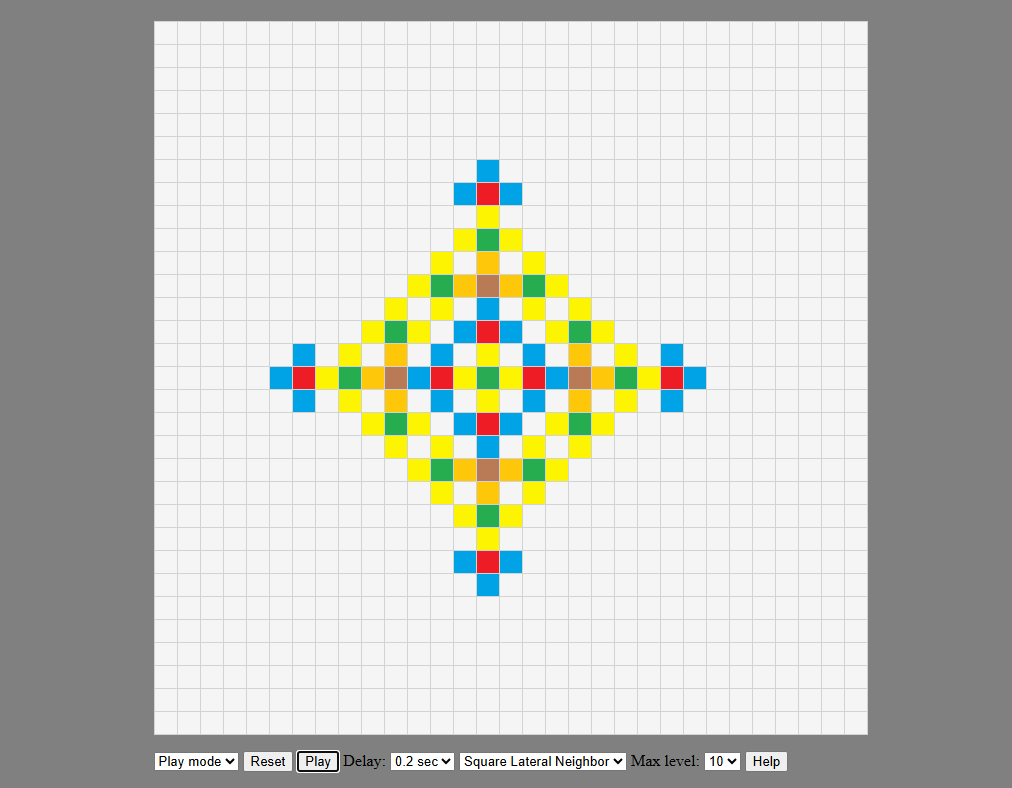
\includegraphics[width=0.75\textwidth]{Sejt_v1.png}
\caption{A sejtautomata, amely 2024-01-21-én íródott, az alsó verzió}
\end{figure}

\begin{figure}[htbp]
\centering
\includegraphics[width=0.8\textwidth]{\detokenize{2024-01-21 23_40_30-Window.jpg}}
\caption{Összehasonlítás a tankönyvvel}
\end{figure}

\begin{thebibliography}{99}
\addcontentsline{toc}{chapter}{\bibname}
\bibitem{varga-geda2024}
Varga, Éva -- Geda, Gábor: \textit{Az interdiszciplinaritás lehetőségei a nyelvoktatás és az algoritmikus gondolkodás területén}. In: Kovács, Enikő (szerk.) \textit{III. Pedagógiai Módszertani Konferencia -- A jövő kihívásainak pedagógiája} absztraktkötet. Eger, Líceum Kiadó, 2024, pp. 48--48.
\bibitem{geda-biro2020}
Geda, Gábor -- Biró, Csaba: \textit{A possible way to develop algorithmic thinking}. \textit{Acta Didactica Napocensia}, 13(1), 2020, pp. 19--28.
\bibitem{cormen2009}
Cormen, Thomas H. -- Leiserson, Charles E. -- Rivest, Ronald L. -- Stein, Clifford: \textit{Introduction to Algorithms}. MIT Press, Cambridge, 2009.
\bibitem{elte-eca}
ELTE Informatikai Kar: \textit{Elementary Cellular Automaton}. Elérhető: \url{http://lambda.inf.elte.hu/ElementaryCellularAutomaton.xml} (megtekintve: 2026.03.18.).
\bibitem{elmasri2016}
Elmasri, Ramez -- Navathe, Shamkant B.: \textit{Fundamentals of Database Systems}. Pearson, Boston, 2016.
\bibitem{fielding2000}
Fielding, Roy T.: \textit{Architectural Styles and the Design of Network-based Software Architectures}. Doctoral dissertation, University of California, Irvine, 2000.
\bibitem{fowler2002}
Fowler, Martin: \textit{Patterns of Enterprise Application Architecture}. Addison-Wesley, Boston, 2002.
\bibitem{gardner1970}
Gardner, Martin: \textit{Mathematical Games -- The Fantastic Combinations of John Conway's New Solitaire Game ``Life''}. \textit{Scientific American}, 223(4), 1970, 120--123.
\bibitem{geda-progmod}
Geda Gábor: \textit{A programozás módszertani alapjai}. Oktatási segédanyag, Eszterházy Károly Katolikus Egyetem, 2023.
\bibitem{ilachinski2001}
Ilachinski, Andrew: \textit{Cellular Automata: A Discrete Universe}. World Scientific Publishing, Singapore, 2001.
\bibitem{kapp2012}
Kapp, Karl M.: \textit{The Gamification of Learning and Instruction}. Pfeiffer, San Francisco, 2012.
\bibitem{krug2014}
Krug, Steve: \textit{Don't Make Me Think}. New Riders Publishing, Berkeley, 2014.
\bibitem{laravel}
\textit{Laravel Documentation}. Elérhető: \url{https://laravel.com/docs/12.x} (megtekintve: 2026.02.27.).
\bibitem{sanctum}
\textit{Laravel Sanctum Documentation}. Elérhető: \url{https://laravel.com/docs/12.x/sanctum} (megtekintve: 2026.03.05.).
\bibitem{martin2008}
Martin, Robert C.: \textit{Clean Code: A Handbook of Agile Software Craftsmanship}. Prentice Hall, Upper Saddle River, 2008.
\bibitem{vonneumann1966}
Neumann, John von: \textit{Theory of Self-Reproducing Automata}. University of Illinois Press, Urbana, 1966.
\bibitem{youtube-cellauto}
Numberphile: \textit{Conway's Game of Life Explained}. YouTube videó. Elérhető: \url{https://www.youtube.com/watch?v=N0jSqWeyeFU} (megtekintve: 2026.04.09.).
\bibitem{react}
\textit{React Documentation}. Elérhető: \url{https://react.dev/} (megtekintve: 2026.03.11.).
\bibitem{richardson2007}
Richardson, Leonard -- Ruby, Sam: \textit{RESTful Web Services}. O'Reilly Media, Sebastopol, 2007.
\bibitem{silberschatz2019}
Silberschatz, Abraham -- Korth, Henry F. -- Sudarshan, S.: \textit{Database System Concepts}. McGraw-Hill, New York, 2019.
\bibitem{sommerville2015}
Sommerville, Ian: \textit{Software Engineering}. Pearson, London, 2015.
\bibitem{typescript-docs}
\textit{TypeScript Documentation}. Elérhető: \url{https://www.typescriptlang.org/docs/} (megtekintve: 2026.04.15.).
\bibitem{wolfram2002}
Wolfram, Stephen: \textit{A New Kind of Science}. Wolfram Media, Champaign, 2002.
\bibitem{wolfram-mathworld-ca}
Wolfram MathWorld: \textit{Cellular Automaton}. Elérhető: \url{https://mathworld.wolfram.com/CellularAutomaton.html} (megtekintve: 2026.02.14.).
\bibitem{kodbazis-php-haladok}
Kód bázis: \textit{PHP tanfolyam haladóknak}. Elérhető: \url{https://kodbazis.hu/php-tanfolyam-haladoknak} (megtekintve: 2025.10.25.).
\bibitem{kodbazis-react-kurzus}
Kód bázis: \textit{React egyszerűen elmagyarázva}. Elérhető: \url{https://kodbazis.hu/react-kurzus} (megtekintve: 2026.03.19.).
\bibitem{kodbazis-javascript-alapok}
Kód bázis: \textit{JavaScript az alapoktól}. Elérhető: \url{https://kodbazis.hu/javascript-az-alapoktol} (megtekintve: 2026.02.15.).
\bibitem{kodbazis-php-alapok}
Kód bázis: \textit{PHP az alapoktól}. Elérhető: \url{https://kodbazis.hu/php-az-alapoktol} (megtekintve: 2024.11.01.).
\bibitem{kodbazis-js-gyakorlo}
Kód bázis: \textit{JavaScript interaktív gyakorló feladatok -- kezdőtől haladó szintig}, 2026.03.29.
\bibitem{laravel-releases}
\textit{Laravel Releases}. Elérhető: \url{https://laravel.com/docs/12.x/releases} (megtekintve: 2026.03.22.).
\bibitem{php-docs}
\textit{PHP 8.2 Documentation}. Elérhető: \url{https://www.php.net/docs.php} (megtekintve: 2026.01.12.).
\bibitem{react-19-blog}
\textit{React v19}. Elérhető: \url{https://react.dev/blog/2024/12/05/react-19} (megtekintve: 2026.03.22.).
\bibitem{vite-guide}
\textit{Vite (TypeScript)}. Elérhető: \url{https://vite.dev/guide/} (megtekintve: 2026.04.05.).
\bibitem{eslint-docs}
\textit{ESLint -- Find and fix problems in your JavaScript code}. Elérhető: \url{https://eslint.org/} (megtekintve: 2026.04.04.).
\bibitem{html5-spec}
\textit{HTML5 Living Standard}. Elérhető: \url{https://html.spec.whatwg.org/multipage/} (megtekintve: 2024.10.12.).
\bibitem{css3-roadmap}
\textit{Introduction to CSS3}. Elérhető: \url{https://www.w3.org/TR/2001/WD-css3-roadmap-20010523/} (megtekintve: 2024.10.26.).
\bibitem{mysql-docs}
\textit{MySQL Documentation}. Elérhető: \url{https://dev.mysql.com/doc/} (megtekintve: 2024.02.10.).
\bibitem{phpmyadmin}
\textit{phpMyAdmin -- Bringing MySQL administration to the web}. Elérhető: \url{https://www.phpmyadmin.net/} (megtekintve: 2025.10.05.).
\bibitem{curl-docs}
\textit{cURL Documentation Overview}. Elérhető: \url{https://curl.se/docs/} (megtekintve: 2026.03.25.).
\bibitem{eloquent-orm}
\textit{Eloquent ORM}. Elérhető: \url{https://laravel.com/docs/5.0/eloquent} (megtekintve: 2026.04.05.).
\bibitem{json-org}
\textit{Introducing JSON}. Elérhető: \url{https://www.json.org/json-en.html} (megtekintve: 2025.12.12.).
\bibitem{cellauto-api-repo}
Borsos László: \textit{Cellauto API backend forráskód}. GitHub repository. Elérhető: \url{https://github.com/f4mqfm/cellauto_api} (Letöltve: 2026.04.22.).
\bibitem{cellauto-admin-repo}
Borsos László: \textit{Cellauto Admin felület forráskód}. GitHub repository. Elérhető: \url{https://github.com/f4mqfm/cellauto_admin} (Letöltve: 2026.04.22.).
\bibitem{cellauto-frontend-repo}
Borsos László: \textit{Cellauto Frontend felhasználói felület forráskód}. GitHub repository. Elérhető: \url{https://github.com/f4mqfm/cellauto_frontend} (Letöltve: 2026.04.22.).
\end{thebibliography}

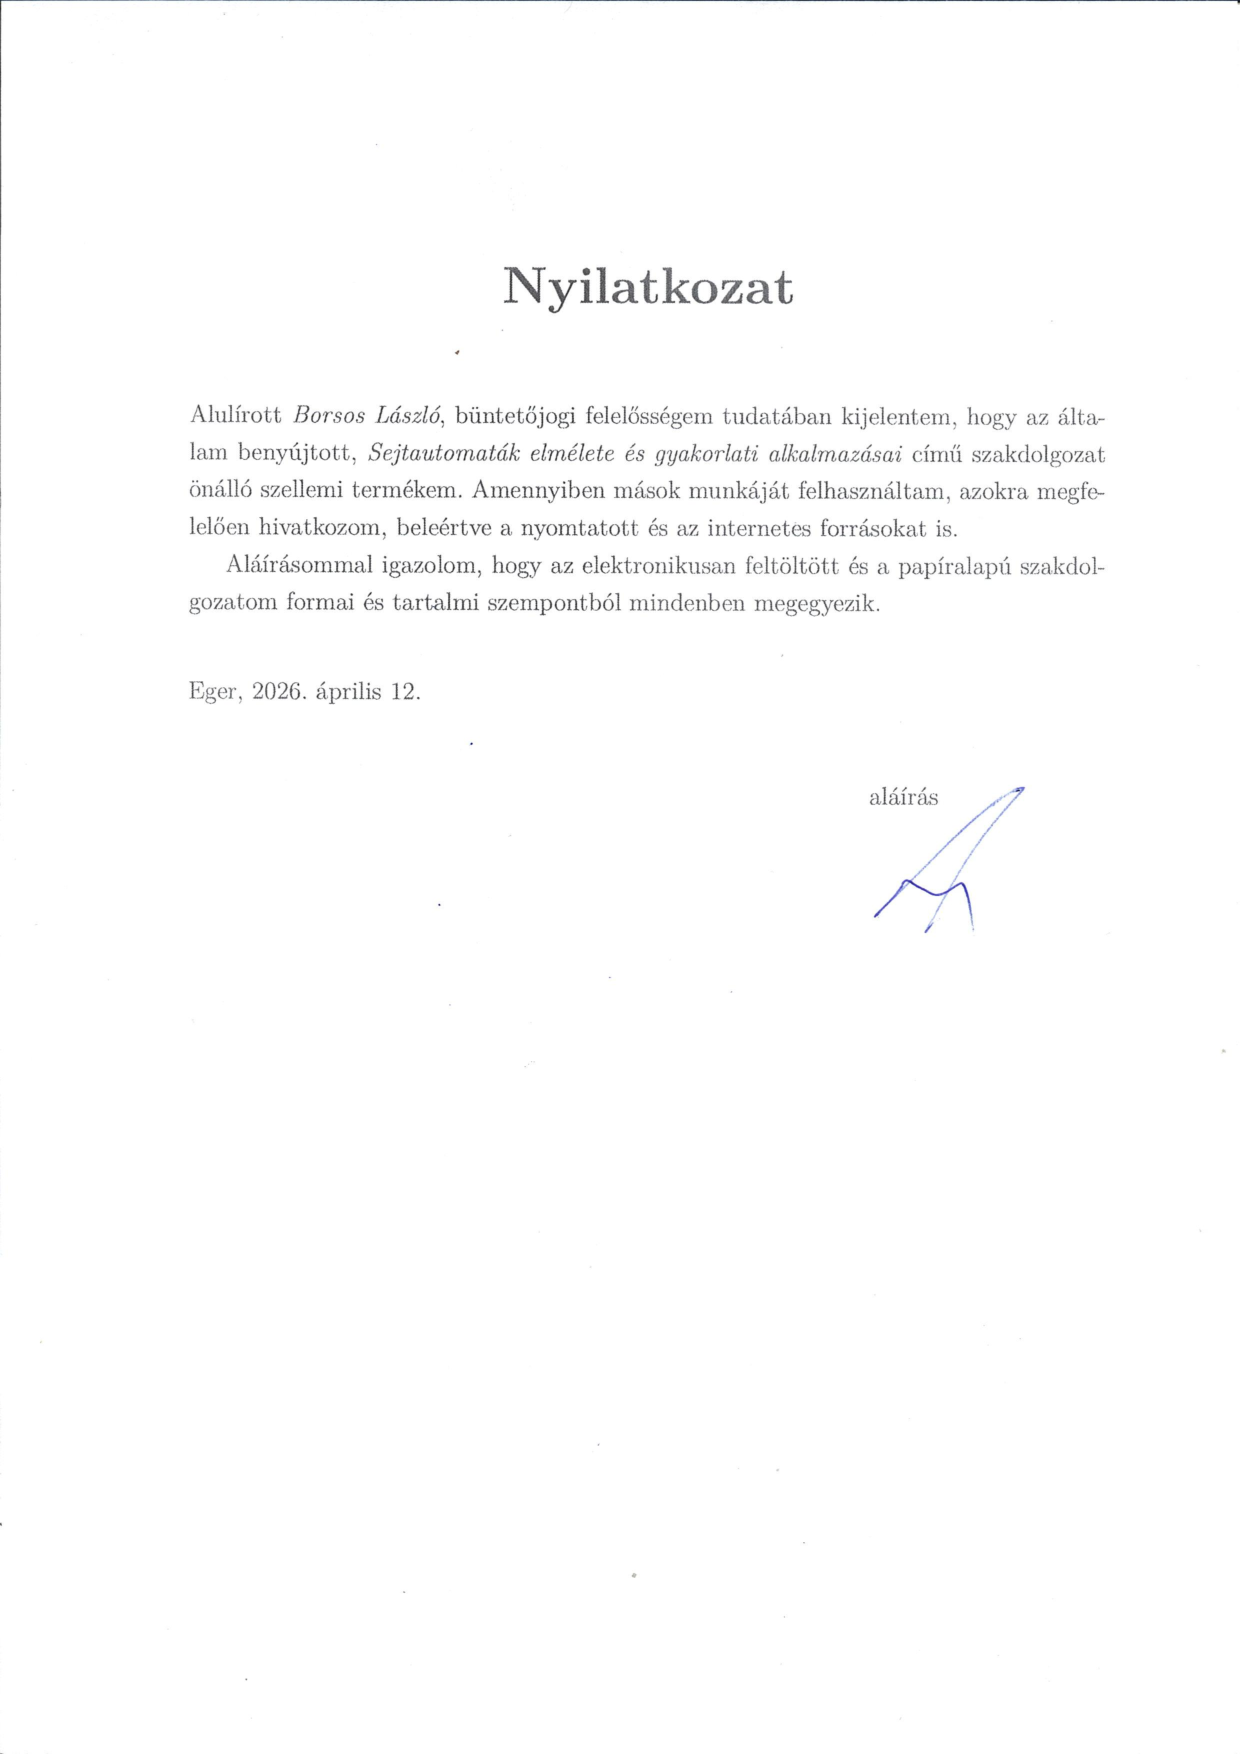
\includepdf[pages=-]{nyilatkozat Borsos Laszlo alairva.pdf}

\end{document}
